\begin{sloppypar}
\section{\cf{\cf{spice-daemon}} ---\hspace{20px} a Python wrapper for SPICE solvers}
\end{sloppypar}
% \cf{spice-daemon} and \cf{qnn-spice}

This chapter introduces \cf{qnn-spice} and \cf{spice-daemon}, python libraries that improve
traditional SPICE environments (such as LTspice) tailored for the design and simulation of
superconducting nanowire devices. \cf{qnn-spice} is a toolkit that helps synchronize and
version track all the models produced by MIT's Quantum Nanostructures and Nanofabrication 
group using the traditional git workflow. \cf{spice-daemon} is a python package that adds 
new functionality such as hyperparametrized models, noise and post-processing to LTspice.

\subsection{SPICE}

One popular way of simulating electronics is using SPICE 
(Simulation Program with Integrated Circuit Emphasis). 
SPICE solvers are an industry standard method of simulation that combines DC analysis (also known as
operating point analysis), AC analysis (linear small-signal frequency domain analysis), and 
transient analysis (time-domain analysis for non-linear differential algebraic equations)
among other analysis methods \cite{spice-og}.

Since then, the original Berkley SPICE
inspired multiple other SPICE solvers including LTspice, a popular free circuit simulator \cite{ltspice-diff-post}. SPICE models for 
superconducting electronics exist including models for the nanowire,
hTrons and Josephson Junctions implemented as SPICE netlists. For nanowires, we
particularly care about transient analysis where the solver
is based on a piece-wise finite method using dynamic timestepping fitted to a 
low-order polynomial \cite{spice-book}.

\subsubsection{Interfacing with LTspice}%Netlists and Schematic Capture}
\label{interfacing_with_ltspice}

Interfacing with SPICE software involves generating a netlist --- a code snippet that defines
how the different circuit elements are connected to each other. Netlists have a \ccf{.net} (and 
sometimes a \ccf{.cir}) extension and can be used across different SPICE implementations. 
Netlists are encoded as ASCII files and as such editing them is straightforward.

Some commercial versions of SPICE
software, including LTspice, add Schematic Capture capability. Schematic Capture allows for a
native GUI encoding of a circuit to be converted into a netlist (in LTspice, that is a 
schematic file with the extension \ccf{.asc}).

LTspice generates multiple types of files after each successful run. The most common type is 
a compressed binary \ccf{.raw} file that is generated after AC and transient simulations. An
optional \ccf{.op.raw} file is also generated that saves the DC solution and can be imported
to skip DC simulation. LTspice also generated a \ccf{.plt} file that encodes the layout of and
variables plotted in the LTspice plotting window. The python package \cf{PyLTSpice}
has built-in methods to read and write RAW files \cite{pyltspice}. RAW files
are the only form of input that can be used by the LTspice waveform viewer.

A \ccf{.log} file is always generated, 
regardless of the type of simulation and/or its success. For a smoother experience using LTspice on Mac with \cf{spice-daemon}, it is
recommended you uncheck ``automatically delete .raw and .log files'' under the operation sub-menu
in the LTspice preferences. This setting is by default checked on Mac (but not on Windows) and
deletes files that \cf{spice-daemon} uses to track LTspice simulations (discussed in section \ref{sd_models}).

SPICE directives refer to text that is passed from the Schematic Capture circuit directly to the netlist.
For example, the \cf{.tran} directive sets up a transient simulation with a specified stop time (and other
optional parameters). If an undefined directive is specified, for example, misspelling \cf{.tarn} instead of \cf{.tran}, it is passed to the netlist normally, and upon running a simulation, a warning is raised
with no effect on the simulation output.

\subsubsection{Models}

Regular SPICE models are composed of two main types of files, symbol (\ccf{.asy}) and library
(\ccf{.lib}) files. A symbol file defines the visual metaphor used by the schematic capture
part of LTspice to visualize the element and its ports. The library file contains the subcircuit
definitions for models. A subcircuit defines how ports connect to each other using other components
or subcircuits. A library file can contain the subcircuits and they can each be referenced individually
by a separate symbol file.

LTspice allows these files to exist in two locations by default. The Model Library folder and the circuit directory. In other words, whenever the LTspice schematic needs to reference a symbol or
library file, unless a path explicitly references a full path, LTspice checks the Model Library folders 
and the parent folder for the schematic. This makes it hard to continuously develop models in a repository
while still being able to use the most up to date version. This issue is addressed in section \ref{qnn-spice}.

% \subsubsection{Transient Simulation}

% \todoidea[inline]{Problem/Why?

% Hard to simulate effects

% Fitting to data

% Complicated analysis toolkits

% Noise/custom inputs

% Device level modeling

% Solution/What?

% Wrapper for spice solvers like LTspice.}

\subsection{Installing \cf{spice-daemon} and \cf{qnn-spice} }

Installing \cf{qnn-spice} and \cf{spice-daemon} can be done by cloning the repositories
and symbolically linking the update bash script and \cf{spice.py} files, from each repository
respectively, to your local \cf{/bin}
directory. For instance using the \cf{ln -s} command to link \cf{\$PATH/qnn-spice/update.sh}
to \cf{spice-update} and \cf{\$PATH/spice-daemon/spice.py} to \cf{sd}, you can invoke
the two scripts from using the two commands \cf{spice-update} and \cf{sd} from the terminal at
any time.
\cf{spice-daemon} can also be installed as a Python package with pip to allow for more
flexible control through python scripts -- this is ideal for more optimized workflows,
large parameter sweeps, niche post-processing types or experiment-simulation hybrid
setups.

\subsection{\cf{qnn-spice}} \label{qnn-spice}

In a collaborative setup where SPICE models might be edited (either continuously or with infrequent small fixes), 
having the ability to track the version of the models is important. One solution is to include a version 
string that the editor updates between revisions. Doing so however, does not handle merge conflicts natively and
does not track file differences -- ``diffs''. From these requirements, the widely used version tracking software git can be
used to track diffs and users will always have to re-download the latest version of the model.

One way to manage models in LTspice is to download them individually and place them in the library folder that contains 
all the base models. However, this can be tedious as it requires repeating the process for each model and your
models can't be version tracked easily. An alternative
approach is to store all the models in the same directory as the circuits and manually download each model as needed. 
This has the advantage of forcing the models to be version tracked in your repository, but it can result in a cluttered 
directory and multiple copies of each model on the system. Both methods don't guarantee that you are using the latest
version of a model.

This is where \cf{qnn-spice} comes in, MIT's Quantum Nanostructures and Nanofabrication group (QNN) has multiple
repositories, each with multiple spice models and different access rights. By having a single repository track every repository containing
SPICE models, a single repository could track all the changes across every model produced by the QNN group and still respect each user's access rights. 
This single repository method takes advantage of git submodules, which track the head of each sub-repository.
A helper update script pulls every submodule and creates symbolic links into LTspice's library folder to each model.
The model library and symbol files to be included are specified in a markdown file at the base of each repository. The main respository tracks the
remotes (location and branch) of each repository using git's built-in submodule branch tracker.

\begin{figure}
    \centering
    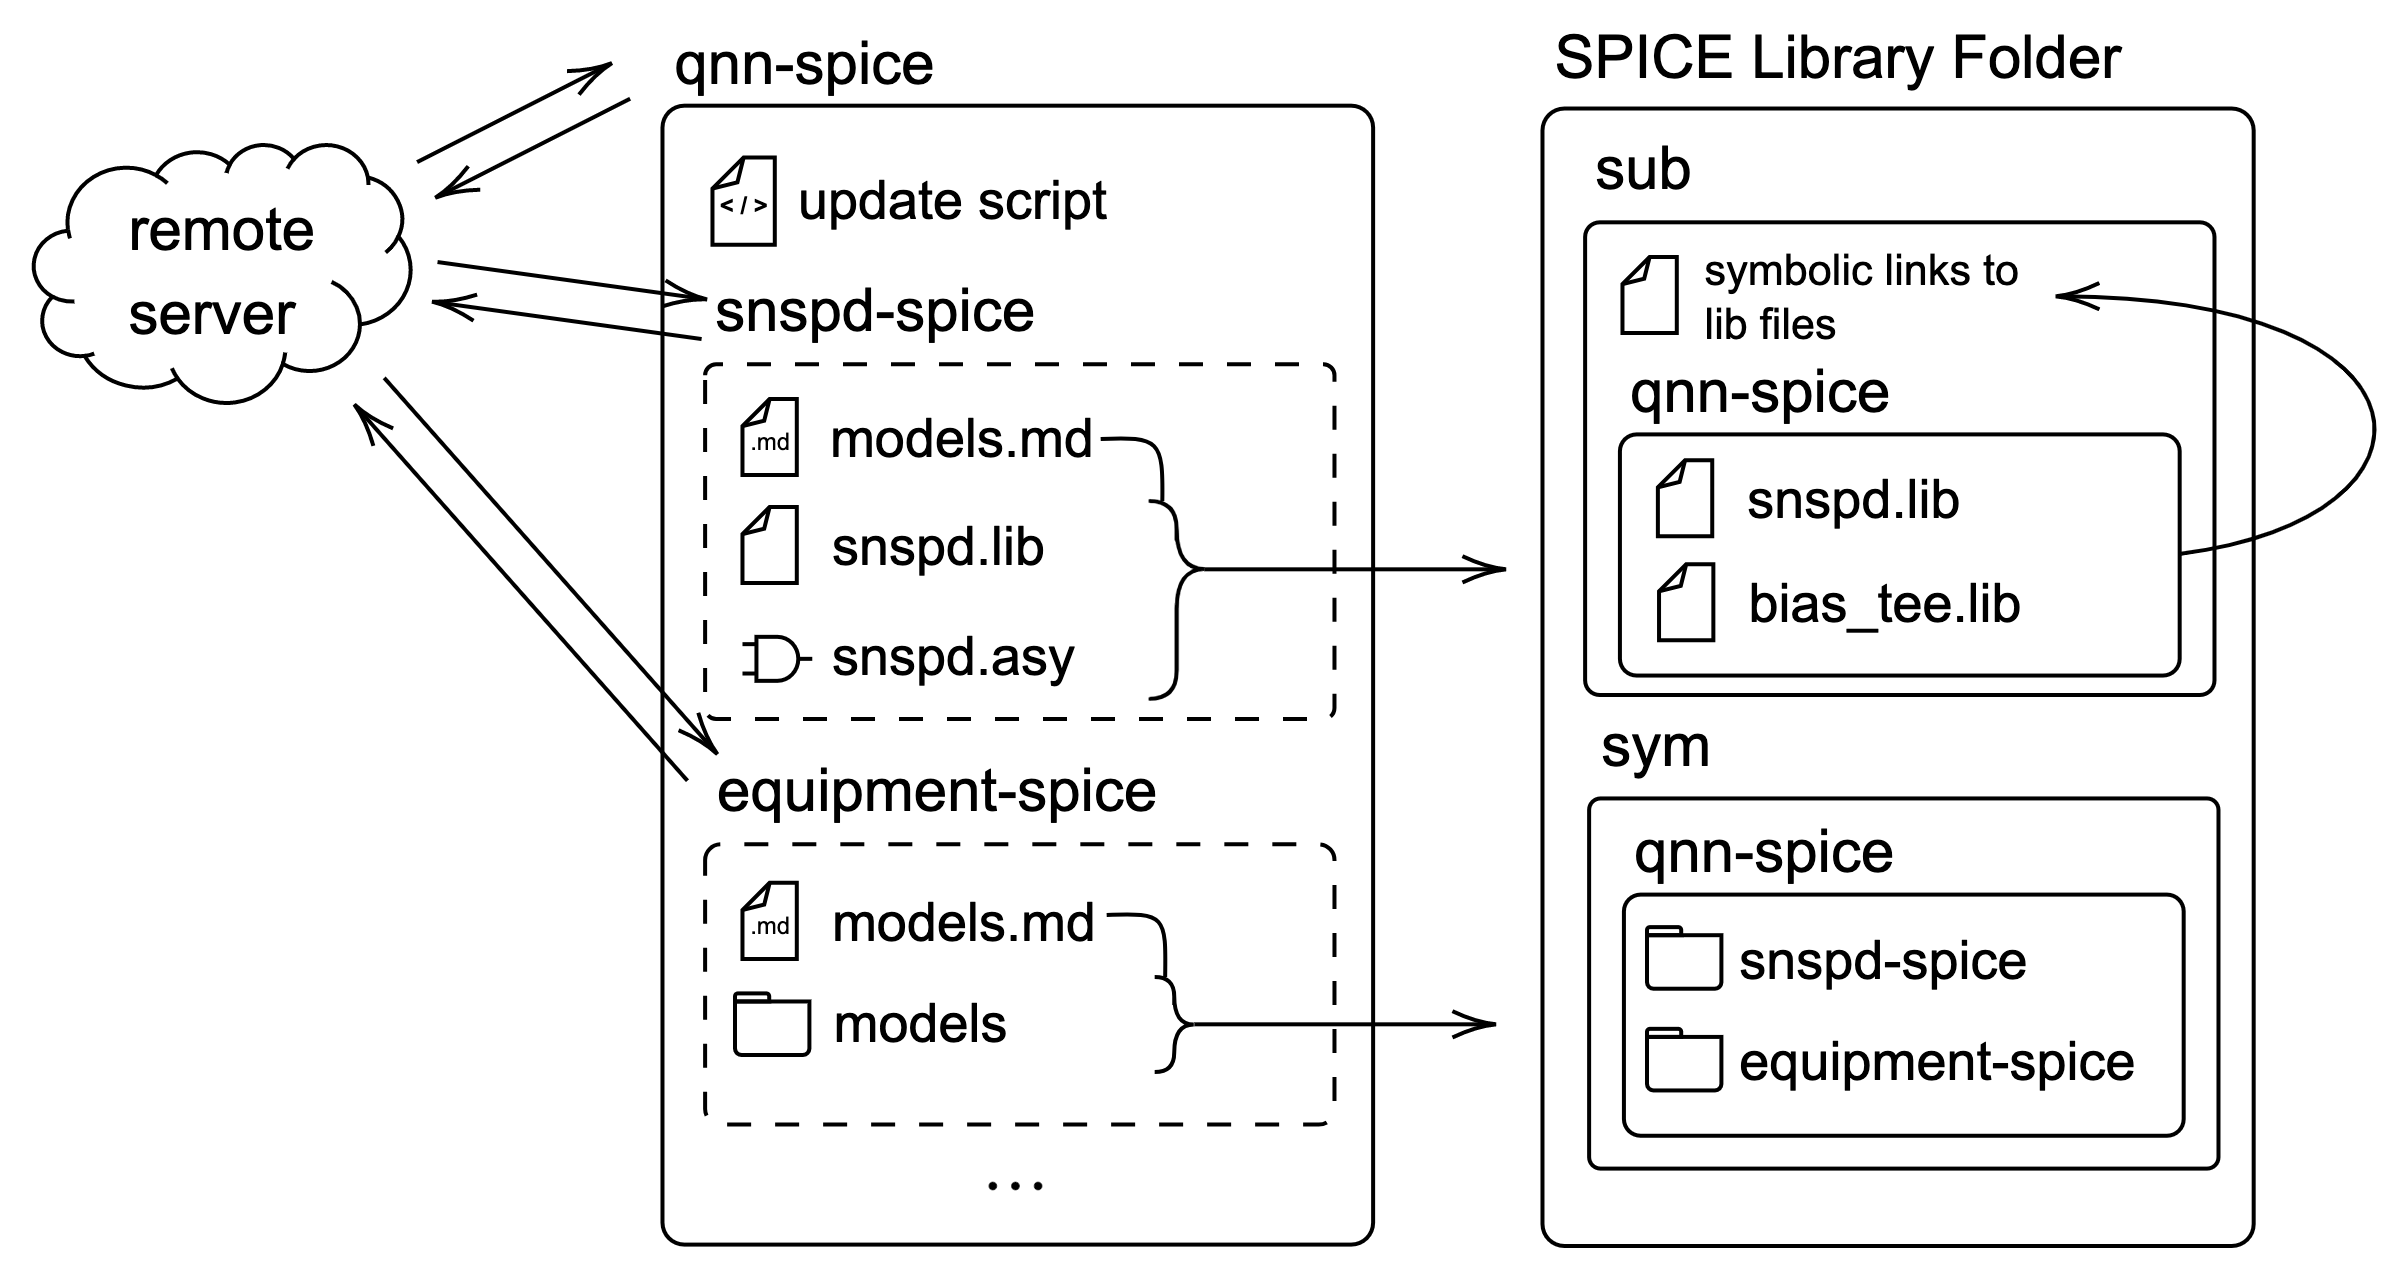
\includegraphics[width=0.7\textwidth]{figs/qnn-spice-interaction.png}
    \caption{A notional diagram of the \cf{qnn-spice} repository and linking to the LTspice Library folder.
    The \cf{qnn-spice} repository tracks the heads (not contents) of multiple git submodules, other repositories version
    tracked using a remote server. The \cf{qnn-spice} update script creates symbolic links from the local
    repository to the Library folder. The folder structure of the submodules (and inner-folders as defined in each submodule's \ccf{models.md} markdown file) is preserved when moving symbol files to the \cf{sym} directory. The folder structure is not necessarily preserved in the library file, it is then flattened by adding another
    layer of symbolic links in the \cf{sub} folder's root to each \ccf{.lib} file.}
    \label{fig:qnn-spice-interaction}
\end{figure}

The use of symbolic links means LTspice is agnostic to where the model was edited from
(locally from the home directory, locally from the model directory or from the remote branch).
When the update script pulls the main and sub repositories, the previous symbolic links are deleted and new ones are 
made. The sub-repository structure is copied into two \cf{qnn-spice} folders are created in the \cf{sub/} and \cf{sym/} 
subfolders of LTspice's library folder. Another set of symbolic links is created in the
\cf{sub/} directory for each file in \cf{sub/\cf{qnn-spice}}. This makes sure that symbol
instances find the referenced subcircuit when they don't reference the parent \cf{qnn-spice}
folder.

The markdown file consists of a list that maps the path of each file to include in the repositories to a destination path in the two
\cf{qnn-spice} subfolders based on their extension. 
The destination path allows users to change the grouping of elements agnostic to how the repositories
were laid out, i.e. you can have two repositories have their elements grouped together and you can split one
repo into multiple folders. 
% \todoidea{how to make a custom module grouping?}

LTspice updates the underlying library subcircuits for models upon every simulation,
and as such you don't need to restart LTspice for this to take effect. However,
it is necessary to restart LTspice to reflect changes in the symbol files. This is 
also applicable to \cf{spice-daemon} dynamic models in section \ref{sd_models} and \ref{dyn_models}.

\cf{qnn-spice} is also capable of merging libs. This means that all the subcircuits can live
on the remote at all times and running a simulation involves redownloading all the 
subcircuits and caching them. This can be done using the \cf{.inc} (include) directive that takes
in the URL for the remote lib. The include directive allows for a built-in way of accessing local
and remote files - it can be used to import remote library files. Every simulation run forces
them to pull (and cache) the latest subcircuits for a model without having to manage this
outside of LTspice. This can be used in \cf{qnn-spice} by invoking the library compiler python script
that compiles a complete library of all subcircuits that are part of \cf{qnn-spice}.
Unfortunately, this doesn't work on the Mac's version of LTspice \cf{17.0} (but does on
Windows and Linux). This feature is useful for continually changing library files in 
a rapid development environment and for syncing models onto new devices without 
any overhead.

% \todoexplain[inline]{Note for updates: lib files automatically updated. Schematic Capture related files (asy) aren't updated.}

\todoexplain[inline]{Include library location? vs. repo loc.}

\subsection{\cf{spice-daemon} assisted LTspice simulations}\label{sd_models}

The main input for \cf{spice-daemon} is a YAML -- a human-readable data-
serialization language -- file that defines simulation parameters, \cf{spice-daemon} models, and
toolkits. A YAML file can also be version tracked, allowing all parameterizations to be known by the host
python script. 
\todoidea[]{cool because u can save runs behind hidden menus and monte carlo things}

\cf{spice-daemon} creates a \cf{Simulation} object for each daemon instance. Each simulation
object has a list of files, \cf{watch\_files}, that are used to indicate the versioning
of a simulation. \cf{spice-daemon} defines a \cf{WatchDog} object whose job is to make sure
\cf{spice-daemon} modules and toolkits are up to date if any of these \cf{watch\_files}
are edited. 
The \cf{WatchDog} module periodically checks for edits on each of the \cf{watch\_files}
and starts a new thread to regenerate some (or all) of the \cf{spice-daemon}-produced files.
For instance, if someone edits an attribute for a component in the YAML specification file, 
the component library file needs to be regenerated to reflect the change in the attribute (but not the symbol file and, depending on the module, the PWL file to be discussed in section \ref{gen_noise}).

Every \cf{Simulation} object defines a couple of important \cf{File} objects that are always present regardless
of the user's setup for LTspice. \cf{File}s are an extension of the Python Standard Library's \cf{Path} object that can additionally:
\begin{enumerate}
    \item track edit timelines,
    \item detect LTspice-native file encodings,
    \item generate dictionaries from YAML files, and
    \item read/write to files.
\end{enumerate}

\cf{spice-daemon} initializes circuits by placing a block that imports a textfile (\cf{trancmd.txt}) 
generated
in the \cf{spice-daemon} data directory. This textfile overwrites SPICE operational variables
(such as \cf{reltol}), defines new \cf{spice-daemon} instantiated parameters and defines the
similation time and step size. This block involves adding text to a schematic and involves
heavy encoding checking when importing the schematic. A failure to encode the data correctly
could result in corrupting the schematic.

\cf{spice-daemon}'s \cf{WatchDog} can be called from the terminal or from a Python script. The terminal
bash script suffices for basic usage of \cf{spice-daemon} intended for non-experimental environments.
When you call \cf{spiced} from the terminal, \cf{spice-daemon} launches the \cf{WatchDog} that checks for 
periodic changes in files, runs the module and toolkit initialization and begins the post-processing logic
accordingly. It also performs a check on the spice schematic (read using \cf{PyLTSpice})
to see if it has been initialized
by \cf{spice-daemon}, if not, it writes a new instantiation block.
\cf{spice-daemon} needs to access simulation parameters - such as simulation time, steps, etc. -
before LTspice starts solving the circuit. This is through \cf{spice-daemon}'s parameter acquisition and injection 
features. 

\cf{spice-daemon}'s main feature is hyperparametrization. It allows for external control
over LTspice variables and circuit topology from a python environment. The topology
based features are discussed in section \ref{dyn_models}. \cf{spice-daemon} allows for 
running large sweeps of data efficiently and allows for producing large datasets
on parameter sweeps using Python's \cf{numpy} and \cf{pandas} packages. This is mostly
intended to be done using the python \cf{spice-daemon} interface where you can automate
both topology, macroscopic parameters and individual element parameters. This is 
an important feature for models that change the underlying differential equation 
coupling such as in nanowires.

While \cf{spice-daemon} was designed for and tested on LTspice, it should work on any
SPICE based simulator and many other non-SPICE simulators. \cf{spice-daemon} has been
used in tandem with Xyce and JosephsonCircuits.jl. For Xyce, and any SPICE-like
simulator that generates files by default, modifying the \cf{watch\_files} allows you
to operate \cf{spice-daemon} normally. For packages such as JosephsonCircuits.jl, you can
trigger \cf{spice-daemon} to run using the python interface provided. This allows
\cf{spice-daemon} to be an abstract wrapper that can help precompute and layout large
networks for any arbitrary circuit simulator.

\begin{figure}
    \centering
    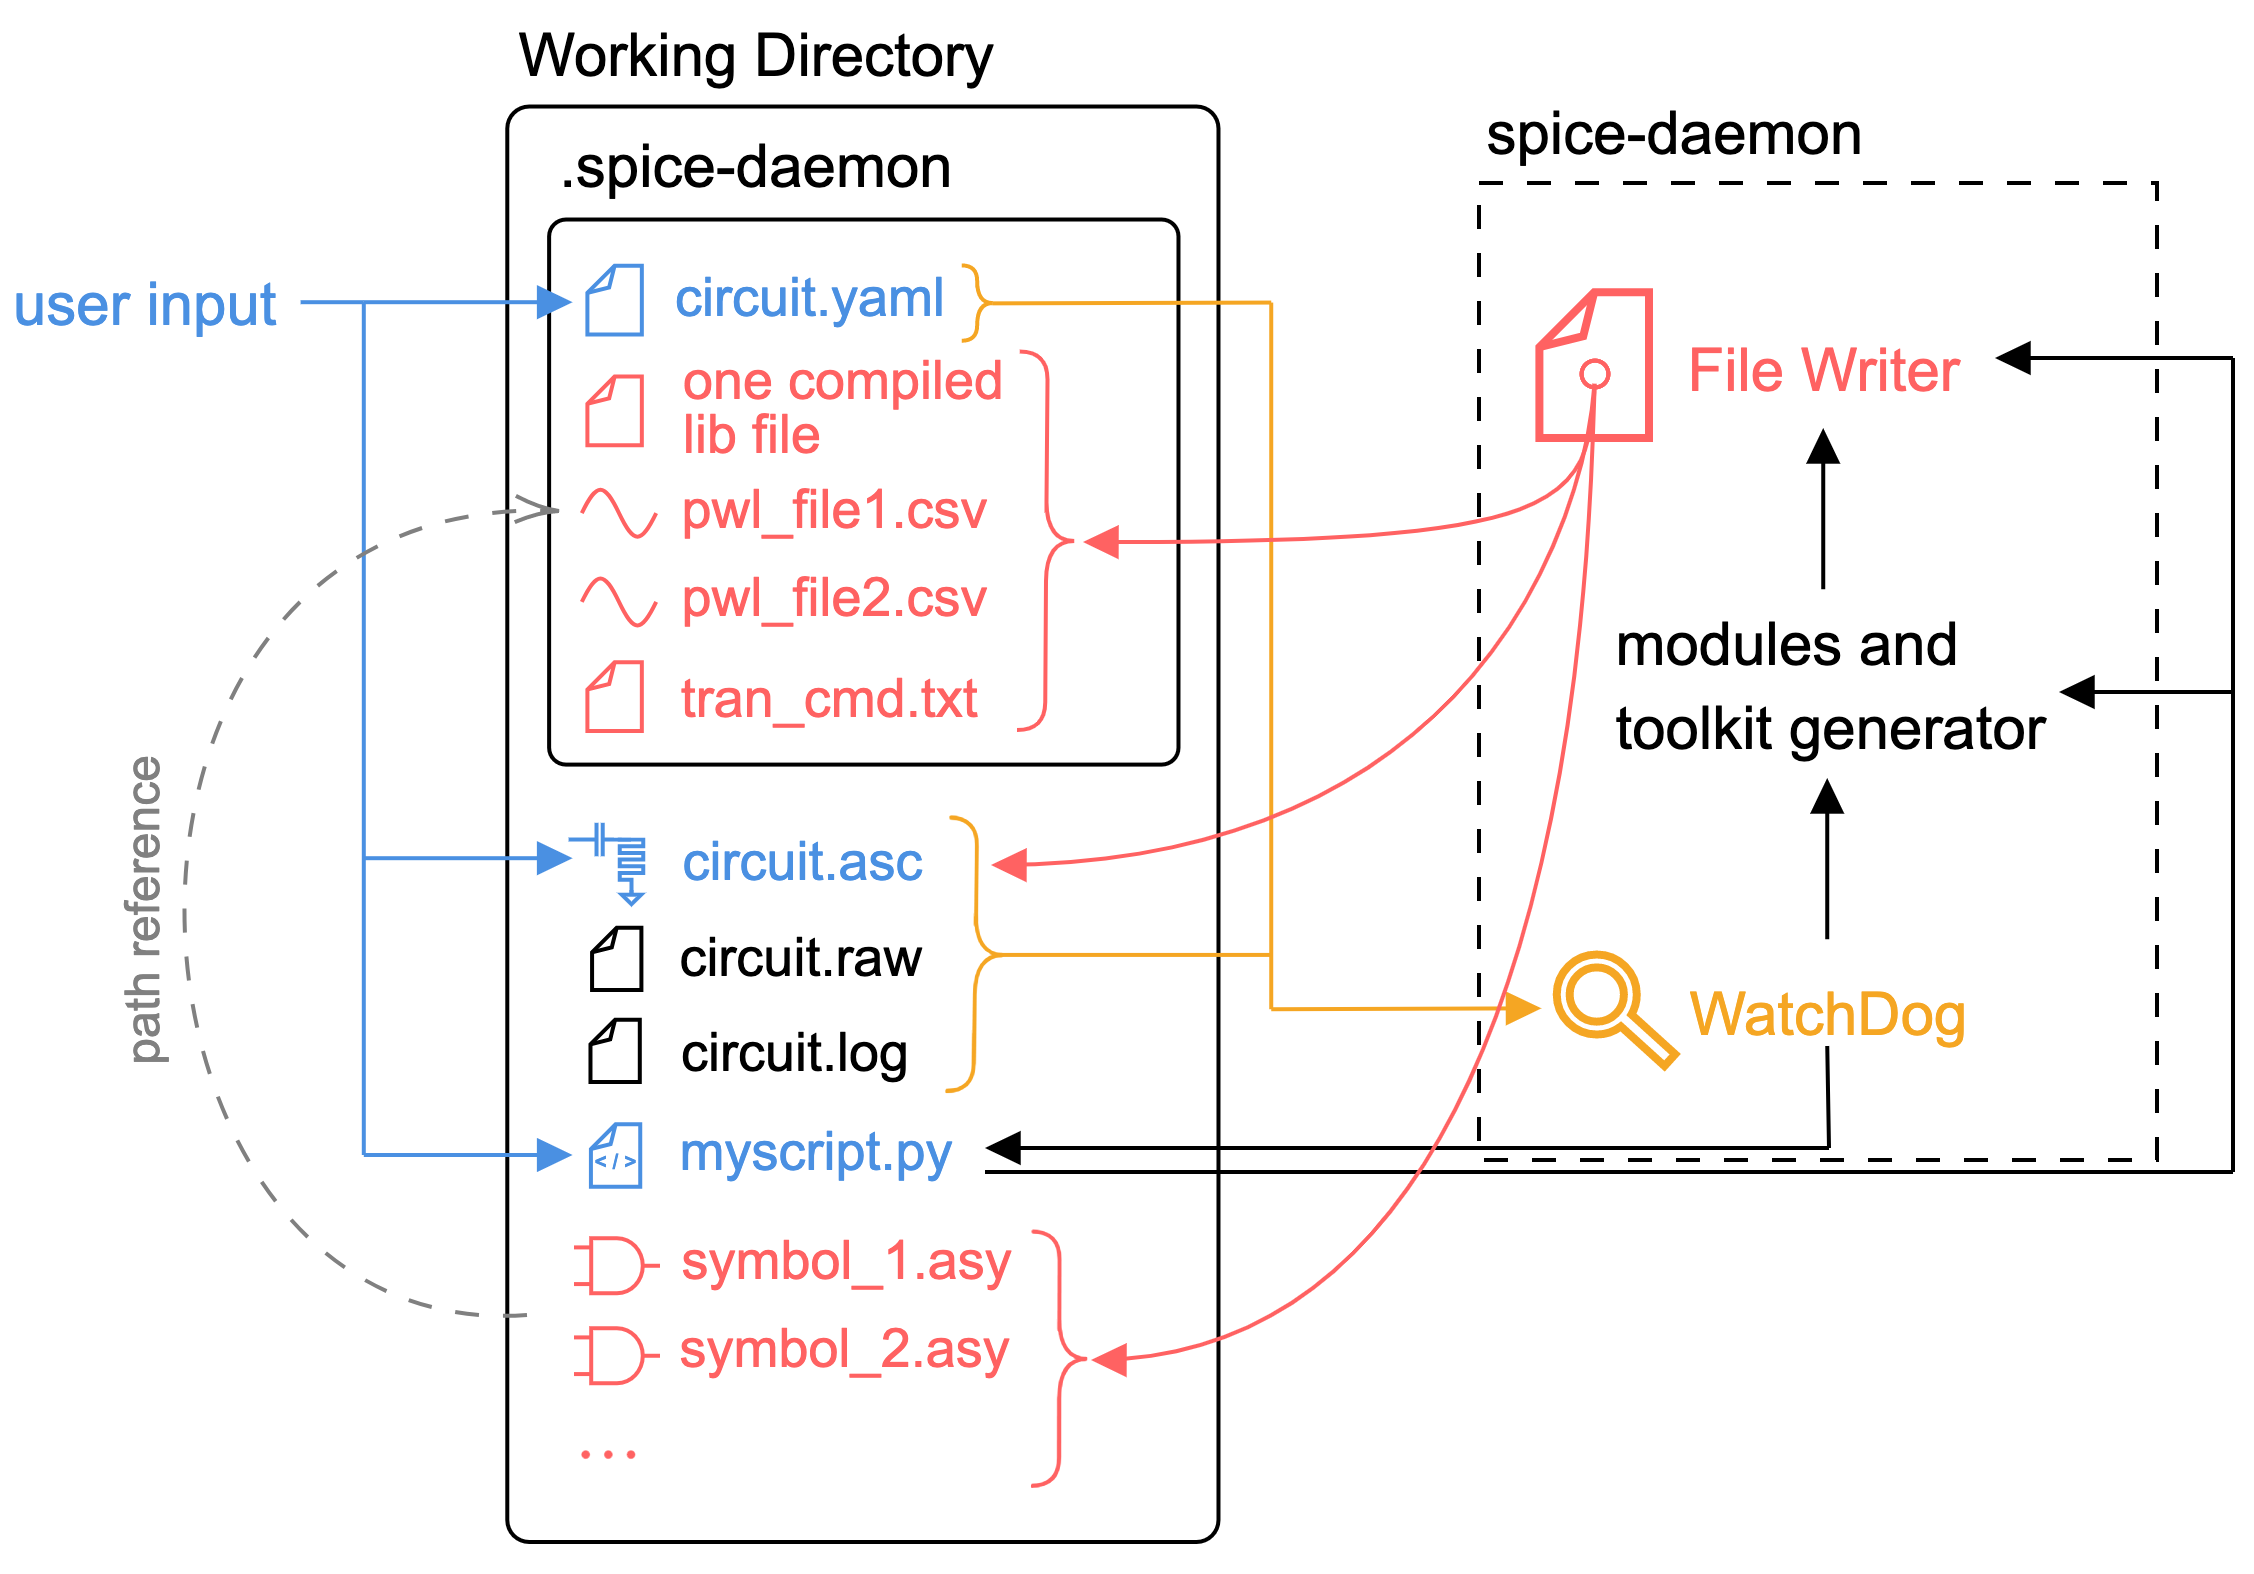
\includegraphics[width=0.7\textwidth]{figs/spice-daemon-interaction.png}
    \caption{Notional diagram showcasing the interaction between different parts of the \cf{spice-daemon}
    library and a typical SPICE workflow. Blue files are edited by the user, this includes: the
    SPICE circuit, a YAML file that defines all the \cf{spice-daemon}-related parameters, and 
    any scripts that use the \cf{spice-daemon} python API. Pink files are generated by spice-daemon,
    this includes: library files, \cf{tran\_cmd.txt}, PWL files, symbol files, and post-processing plot exports. The \cf{WatchDog} module watches for changes in the orange files, including LTspice generated files and user-input enabled files, and triggers module and toolkit regeneration.}
    \label{fig:spice-daemon-interaction}
\end{figure}

In summary, LTspice generates multiple files during every run (discussed in section \ref{interfacing_with_ltspice}). \cf{spice-daemon} is launched in parallel with your circuit
and tracks the edit history of the log file,
the YAML specification file, and the 
circuit schematic using a \cf{WatchDog} object. Based on the edit history, \cf{spice-daemon}
can infer what files have to be regenerated.

\todoidea[inline]{Setting up a simulation, how is tran command and stepping handled}

\todoidea[inline]{setting up a \cf{spice-daemon} simulation}

\todofig[inline]{Diagram of the listen and write files}

% \subsection{Handling Simulation Parameters}

% \cf{spice-daemon} creates a \cf{trancmd.txt} file in the \cf{.\cf{spice-daemon}-data} directory that contains
% the simulation time and steps parameters as well as other user (or daemon) specified simulation parameters.
% This file contains all the 

\subsection{Dynamic Models} \label{dyn_models}

LTspice components are able to be parameterized using a constant global parameter space that can be used when
math expressions are being evaluated (such as the output voltage of a behavioral source or the inductance 
of an inductor). \cf{spice-daemon} adds the ability to hyperparameterize components beyond expressions by granting the
ability to create a PWL file and modify the netlist (circuit topology) of the model between runs.

\subsubsection{Lumped Element Transmission Lines and Tapers}\label{tapers_section}

One type of dynamic model that is incorporated into \cf{spice-daemon} is lumped 
element transmission lines. Instead of using LTspice's built-in transmission
line models (either the Lossless Transmission Lines (T elements) or the 
Lossy Transmission Lines (O elements)), \cf{spice-daemon} allows you to specify a
variable discretization length lumped-element version. 

The Lossless Transmission Line model has a bunch of limitations: it models only one propagation mode,
 does not support non-linear response functions, and does not 
model the DC behavior correctly. The Lossy Transmission Line also suffers from multiple caveats:
it does not support frequency dependence for loss and it also does not support non-linear response 
functions \cite{ltwiki_tline_issues}. This has been recognized by members of the 
LTspice modeling community and a separate frequency based modeling method was developed
for PSpice and LTspice based on the telegrapher's method \cite{camron_model_tline}. Unfortunately, the LTspice
Laplace method in transient analysis is highly unstable and this causes simulating 
more than 1 transmission line impractical. For repeating geometries where accuracy is important, simulating the
transmission lines as a repeating sequence of lumped elements will guarantee the best
convergence and stability.

Another drawback of built-in transmission lines is that 
SPICE programs will have more trouble converging on a correct solution. 
The inclusion of a transmission line introduces new breakpoints at the beginning of the simulation since no timestep during the simulation should be more than the delay of a
transmission line. Including multiple transmission lines of different delays makes the 
situation worse and the number of breakpoints added becomes impractical to simulate (it grows with the 
greatest common multiple of all transmission line delays) \cite{spice-book}.
As a result, you shouldn't use transmission line concatenation to model tapers
as the timestepping algorithm will take impractically long to simulate.

For well-defined convergence with non-convolution based models, we need to be able to simulate repeating
lumped element models from within LTspice. 
However, this would involve laying down thousands 
of repeating chunks of elements manually. One use of dynamic models is generating a model 
that encodes variable length logic. In this method of programming a lumped element transmission
line, the circuit topology can be parametrized by a single parameter in the configuration file 
(in this case number of nodes). This type of automation is not possible using LTspice's built-in
parameterization as the SPICE parameter resolver is queried after topology checks.

This method of simulating a transmission line not only solves the issues introduced by the
T and O models, but also gives us the ability to simulate more complicated transmission lines.
For instance, inductors on a transmission line can be non-linear, making simulating a superconducting
transmission line more accurate. Other possibilities that aren't possible in the LTspice environment
include adding custom elements instead of a repeating sequence of inductors and capacitors allowing us to
model JTWPAs of variable length easily.

Another extension to this one-to-many mapping for the transmission line can be extended to model
lumped-element tapers. The transmission line models in LTspice work for lines with constant 
parameters (impedance, propagation velocity, loss, etc.). With a lumped element model that is fully
controlled by \cf{spice-daemon}, changing the impedance of one port can map the inductance and capacitance
of each finite element to a pair of values based on the taper geometry chosen. This adds another layer
of abstraction where we can define an impedance-matched transmission line with a Klopfenstein geometry
between two impedances $Z_{in},\, Z_{out}$. If we change $Z_{in}$, the \cf{spice-daemon} instance calculates
new tapering parameters smoothly perturbing the impedance of the line from $Z_{in}$ to $Z_{out}$ and
updates the library file for the taper element. 
When LTspice runs a new simulation, it pulls the latest
lib file with the new impedance-matched taper. This non-uniform version of the transmission line
is included as a separate taper model in \cf{spice-daemon} that has additional logic pertaining to 
impedance-matching geometries.

Figure \ref{fig:taper_pnr} showcases the use of a \cf{spice-daemon} generated
taper element to perform Photon Number Resolution on a nanowire strip. 
Figure \label{fig:taper_circ} showcases 4 nanowire elements, mimicking
a single nanowire element recieving up to 4 separate photons. The nanowire
elements are connected to an impedance matching klopfesntein taper of 1000
elements generated by \cf{spice-daemon}. A noise source as described in section
\ref{gen_noise} is connected in parallel to the nanowires. Figure \ref{fig:pnrgobrr}
shows the simulation output for photon number resolution using tapers with 
and without noise.

\begin{figure}
    \centering
    \subfigure[]{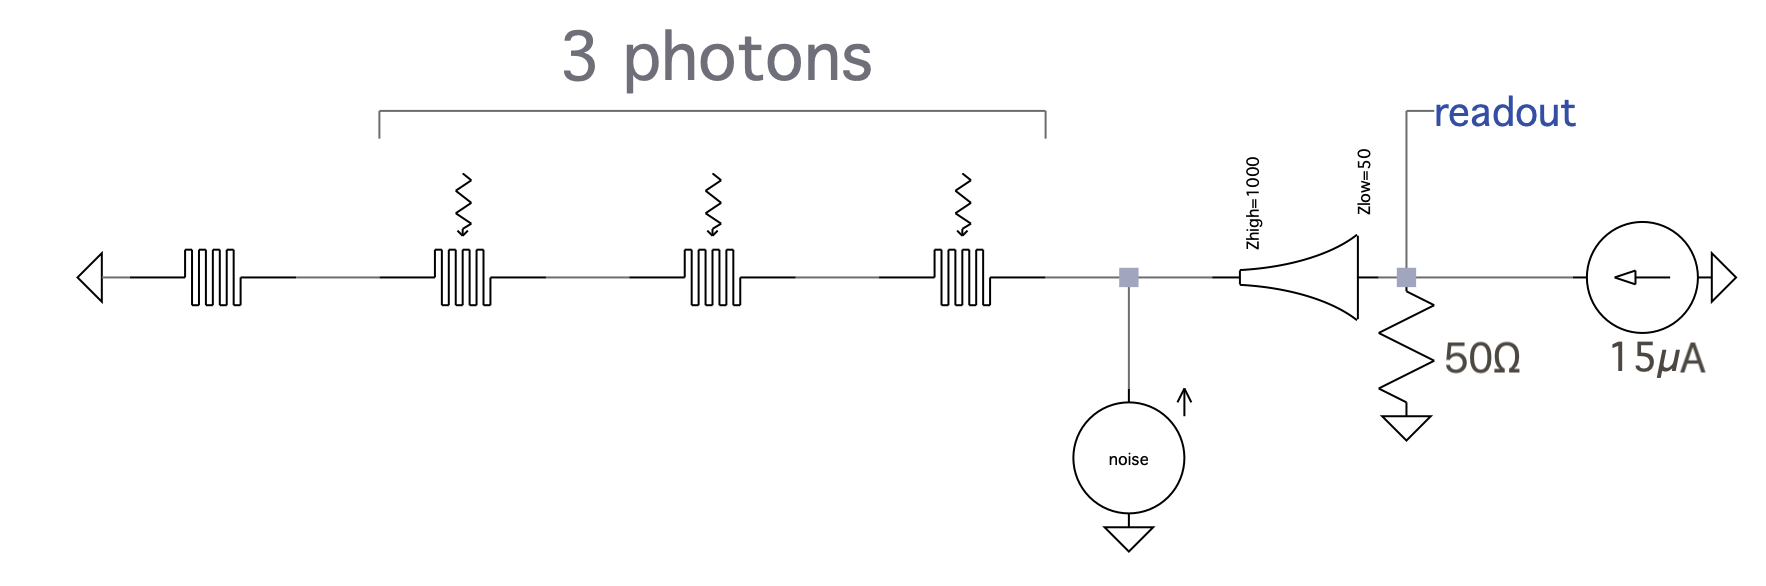
\includegraphics[width=0.8\textwidth]{figs/taper_circ.png}\label{fig:taper_circ}}
    \subfigure[]{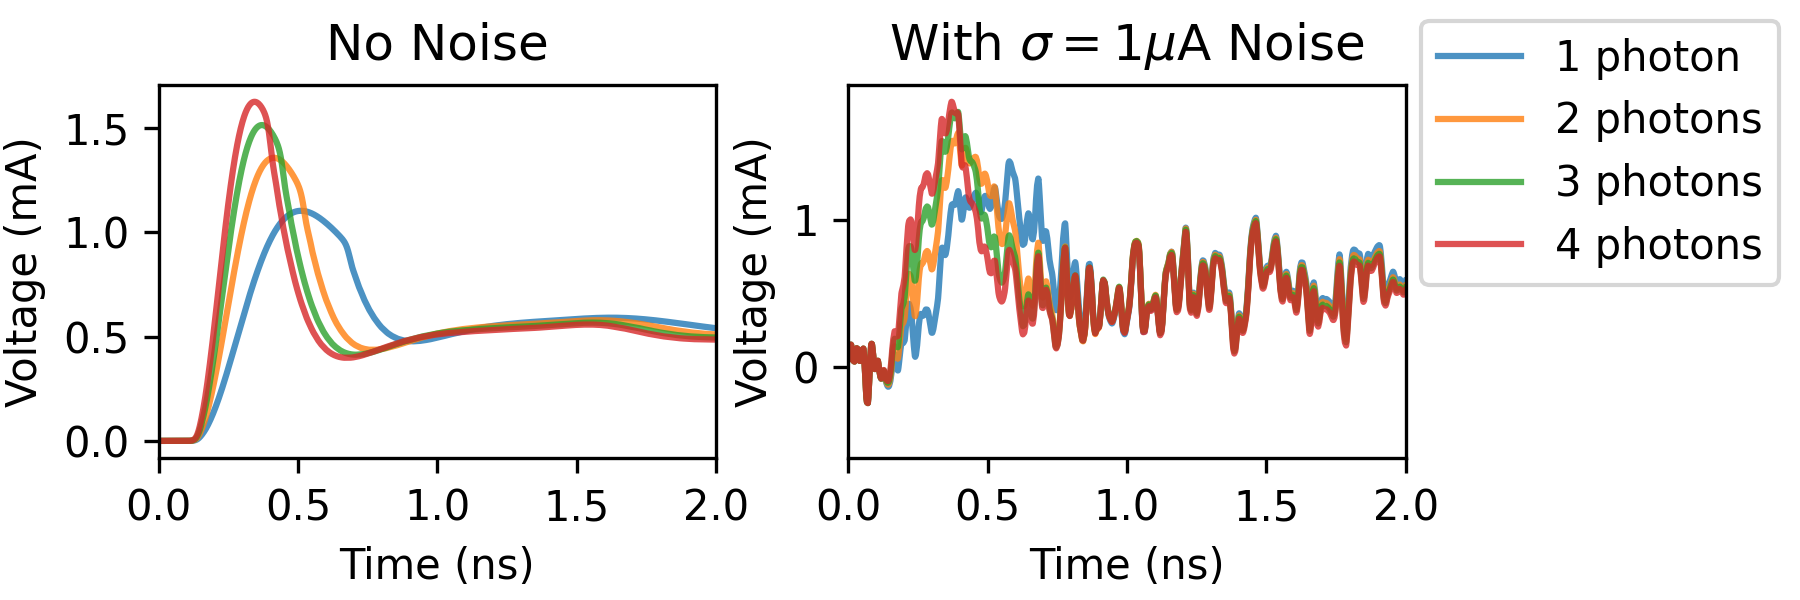
\includegraphics[width=0.8\textwidth]{figs/tapers.png}\label{fig:pnrgobrr}}
    \caption{A \cf{spice-daemon} assisted SPICE simulation of photon number resolution on an SNSPD.
    (a) Illustration of 4 nanowires elements in series that are simulating one 
    effective nanowire with 16
    possibilities of a photon incidence. These elements have no delay between them, making
    them a simpler model that doesn't account for microwave properties of a nanowire.
    The nanowire elements are connected to a \qty{1}{\kilo\ohm} to \qty{50}{\ohm} taper
    biased by \qty{15}{\micro\ampere}. A gaussian noisy current source is added after the taper to
    roughly simulate noise a nanowire might experience.
    The taper and noise source are dynamic models generated using \cf{spice-daemon}.
    (b) Measurement at the circuit readout showcases our ability to resolve the number of
    photons incident on the wire using a taper. When the system experiences noise, the
    margin between photon counts more than 2 gets slimmer.}
    \label{fig:taper_pnr}
\end{figure}

\todoidea[inline]{PNR!}

\todofig[]{pnr}

\subsubsection{Generating Noise} \label{gen_noise}

\todoref[]{somewhere: cite adam_noise}
\todoref[]{@INPROCEEDINGS{8990925,
  author={Qu, Ashley and Zhu, Di and Berggren, Karl K.},
  booktitle={2019 IEEE International Superconductive Electronics Conference (ISEC)}, 
  title={Noise Contribution to Switching Current Distributions in NbN Nanowires}, 
  year={2019},
  volume={},
  number={},
  pages={1-3},
  doi={10.1109/ISEC46533.2019.8990925}}
  }

The ability to add various types of noise when designing superconducting nanowire devices is necessary in order to achieve realistic operation margins and understand the sources of noise in the device. There are multiple types of noise distributions that can couple to nanowires from various sources: gaussian distributions as Johnson noise, Poisson noise
as random photon events and $1/f$ noise due to device-specific microscopic degrees of freedom \cite{1overfinsc}. The simulation, fabrication and testing process of a device
when accounting for noise on each level can inform each step in the process, making noise
simulation essential. The noise model used in a simulation informs the geometry to be 
used in fab and through testing you can identify pitfalls of the noise model used
in simulation.


Since we care about the non-linear transition between
the superconducting and normal state, the addition of noise severely limits the operational margin and
maximum performance of our device. In the example of using an SNSPD, optimal operation of the device 
requires it to be biased at $i_c-\varepsilon$, where $\varepsilon$ is a factor that correlates the 
magnitude of noise and the rate of dark counts (false switching events). For instance, assume the current source is noisy and generates
gaussian noise centered around $0$ with a standard deviation (magnitude) of $\sigma$.
If we bias using $\varepsilon = 2\sigma$ that means $2.28\%$ of all detected counts are dark counts caused by this noise distribution.
Alongside the noise constraint, the signal being measured 
must always be greater than $\varepsilon$ to cause a detection event.

The generation of uncorrelated noise is important for device characterization and
noise source investigation.
While there are methods for generating uncorrelated noise for a simulator, 
LTspice uses one global random number generator causing distributions to be 
inherently correlated.

In transient analysis, we can use a behavioral voltage source with LTspice native math commands
to generate noise such as \cf{random} and \cf{white}. However, LTspice noise commands
generate noise that is correlated amongst instances and is not gaussian in nature. One workaround that was
adopted by the LTspice community involves the Central Limit Theorem \cite{CLM-ltspice}. By using 4 voltage sources each producing a shifted seed for 
gaussian noise (guaranteeing that the seed does not overlap with the simulation time),
the noise sources are uncorrelated. By adding the
outputs of the behavioral voltage sources, the noise distribution approaches that of
a gaussian distribution via the Central Limit Theorem. Note that the number 4 was picked due to a trade-off between the complexity of generating and simulating
that noise and how gaussian it is -- the more sources there are, the more gaussian the noise distribution is.

Another workaround is to use PWL files. PWL files allow you to input piece-wise linear functions into LTspice
sources that are not necessarily behavioral. The PWL operation mode maps (time, value) pairs to a continuous 
output value based on the simulation time. However, if a simulation has $N$ timesteps, $N$ noise points need to be generated to prevent extrapolation.
However, running the simulation with a different number of points can change the number
of timesteps taken and therefore this requires verifying that the numbers are in agreement.
The process of re-creating this noise file, ensuring there are enough data points as timesteps and that the noise data follows a certain distribution is tedious.

To solve this issue, \cf{spice-daemon} can handle the creation of noise sources and their accompanying PWL files,
abstracting them behind a symbol file. The user defines a noise source type (voltage or current), the 
noise distribution it should follow (Poisson, Gaussian, $1/f$, etc.) and distribution parameters (mean, 
standard deviation, etc.). The \cf{spice-daemon} instance then generates a symbol file for a noise source that 
references a sub-circuit for each noise instance. Each sub-circuit references a 
separate PWL file that encodes a list of (time, value) pairs generated in Python using
\cf{NumPy}. As a result, we know that the noise inputs to LTspice actually follow a specific distribution, and we
can verify that the correct noise distribution is being simulated inside LTspice.

This method  allows us to easily have multiple non-correlated noise sources each with an 
arbitrary noise  distribution. Each source has a separate symbol and the noise 
distributions are recalculated after each simulation under the invocation of the \cf{WatchDog}
class. A \cf{spice-daemon}-generated current noise source is included in the photon number resolution 
example showcased in figure \ref{fig:taper_pnr}.

\todo[]{noise example}

\subsubsection{Creating a new dynamic model -- an SNSPI}

This section will walk through making an SNSPI dynamic model to highlight the benefits
of hyperparametrization and serve as a tutorial for extending the \cf{spice-daemon} dynamic model library. 
An SNSPI as discussed in section \ref{snspi_intro} can be thought
of as a non-linear transmission line that exhibits the same switching properties of a nanowire
locally. As a result, an SNSPI can be modeled in the transmission line lumped element picture
(advantages of lumped over built-in O- and T-models discussed in \ref{tapers_section})
using nanowires instead of inductors as shown in figure
\ref{fig:snspi_tline}. In the superconducting regime, they act as a non-linear
inductor and can locally become resistive upon a photon event.

\begin{sloppypar}
The \cf{spice-daemon} module template has 3 base functions defined: (1) \cf{update\_PWL\_file},
(2) \cf{lib\_code} and (3) \cf{generate\_asy\_content}. Function (1) is used to generate 
and write PWL file data that is synced to the simulation timesteps. Function (2)
generates the SPICE library code that controls the electrical behavior of your model.
Function (3) generates the symbol file that is used to draw the model's metaphor. This
section will go through modifying the second function and leaves (1) and (3) unchanged
from the template.
\end{sloppypar}

To develop a module, first define the hyperparameters involved to design your module.
The five degrees of freedom the distributed SNSPI model will simulate will be: (1) the
critical current $i_c$, (2) inductance per unit $L$, (3)capacitance per unit $C$, 
(4) the number of discretization
\cf{num\_units}, (5) the incident photon locations and times (a one-to-many map from incidence 
location to incidence times). This information is input through the YAML file.

We can then append a new SPICE netlist line for each nanowire and capacitor to generate the
meander, making sure the first and last elements connect to the \cf{PINS} defined in the 
class. Since we are using the nanowire model, we need to include the lib file containing
the nanowire definition (synced using \cf{qnn-spice}) using the \cf{.lib} directive. This is
handled automatically (added for every instance) if you are using the \cf{Element.*} 
class to add the components
(with duplicate declarations removed at compilation).
Note the
Berggren et al. nanowire model is a 4 terminal device, where 2 ports are the photon inlet/outlet
and the other 2 are the electrical contacts for the nanowire \cite{karl_spice}. 

\begin{figure}
    \centering
    \subfigure[]{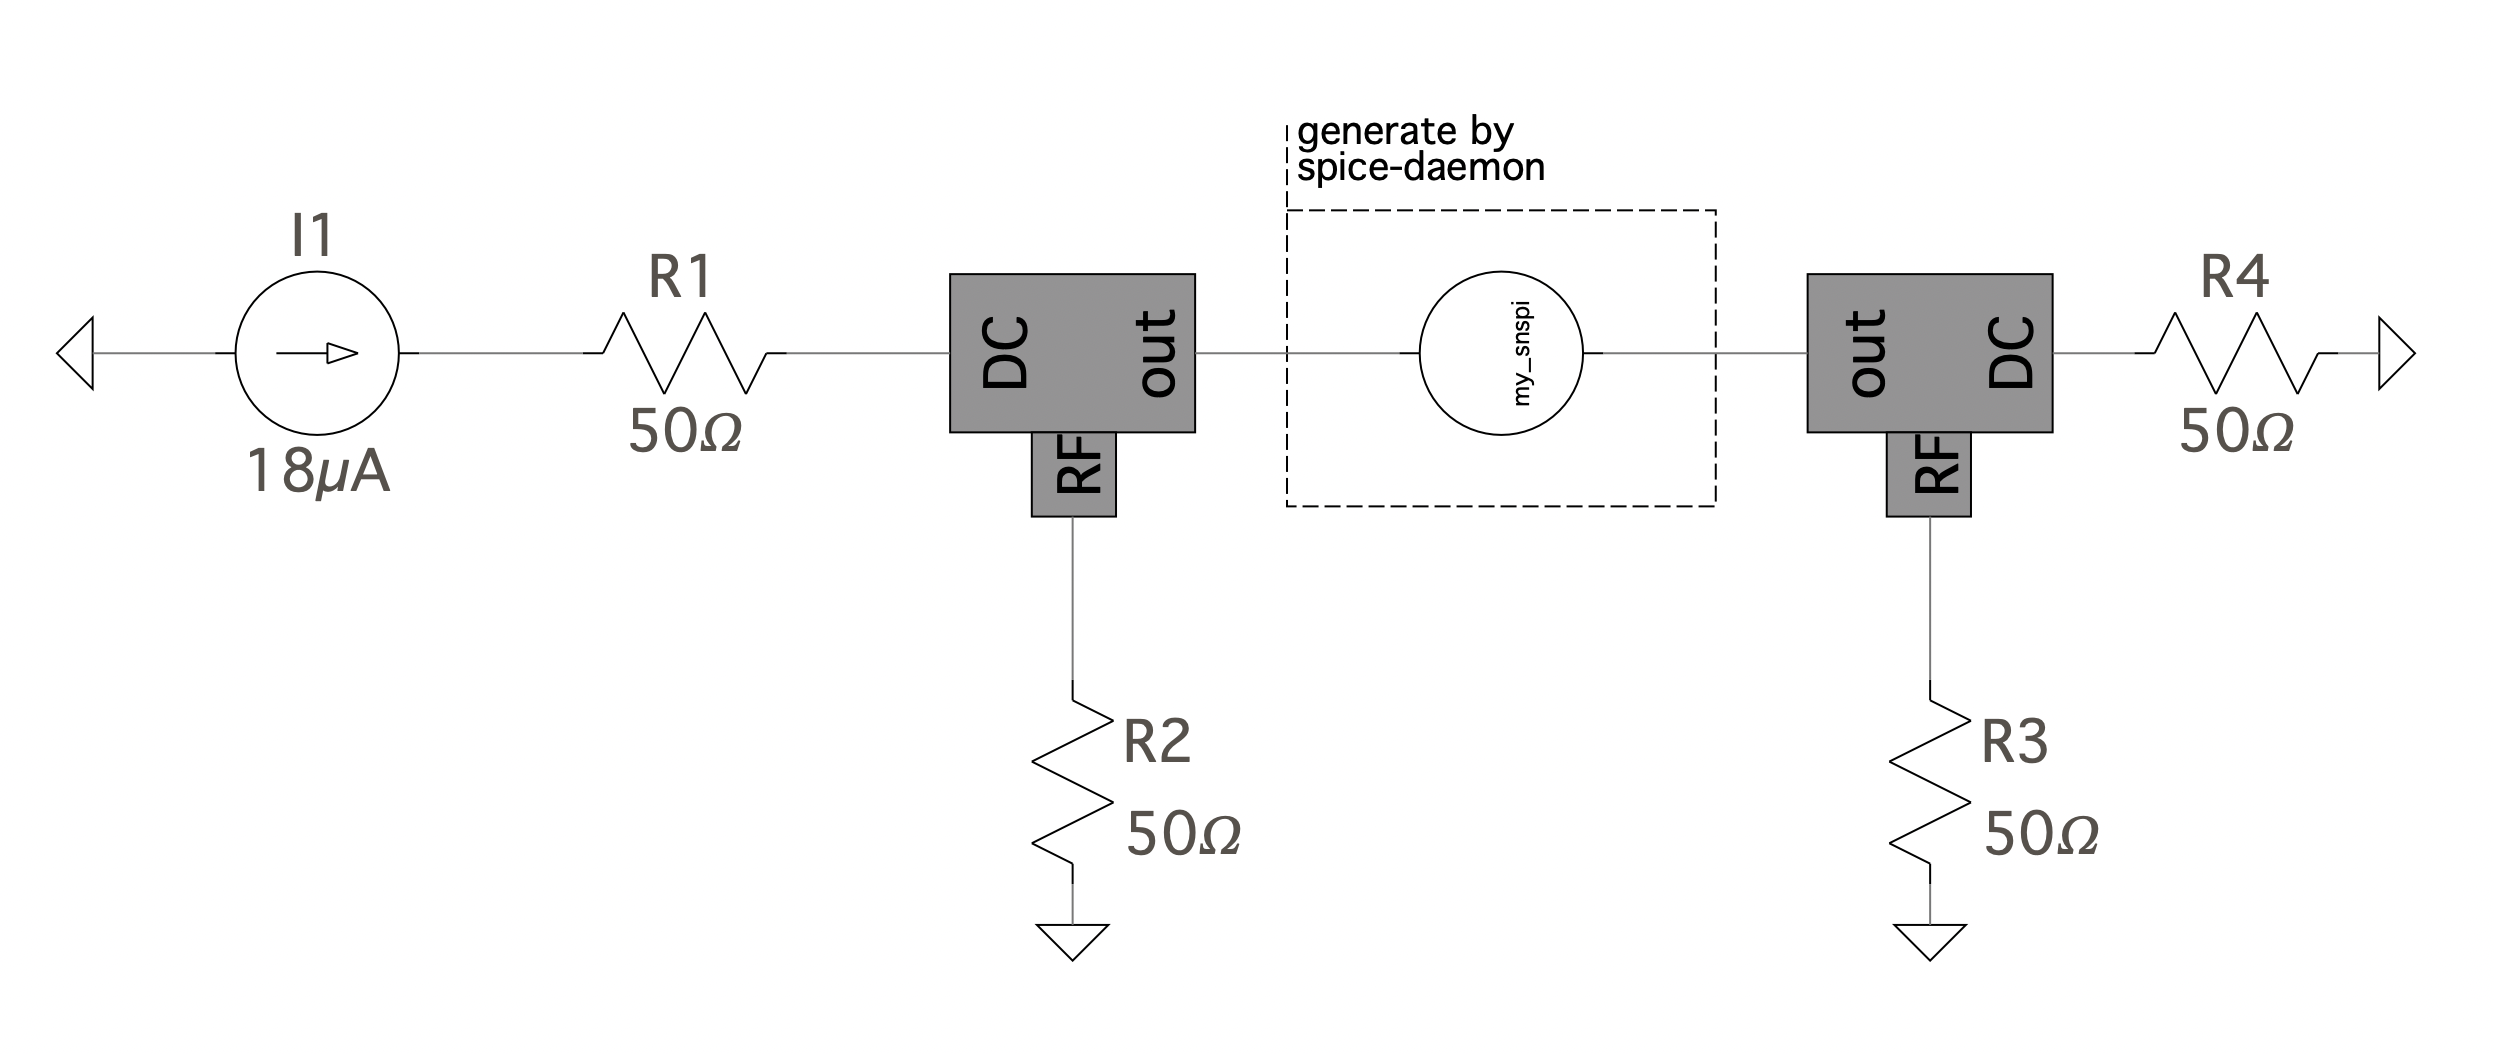
\includegraphics[width=0.49\textwidth]{figs/snspi_circ.png}}
    \subfigure[]{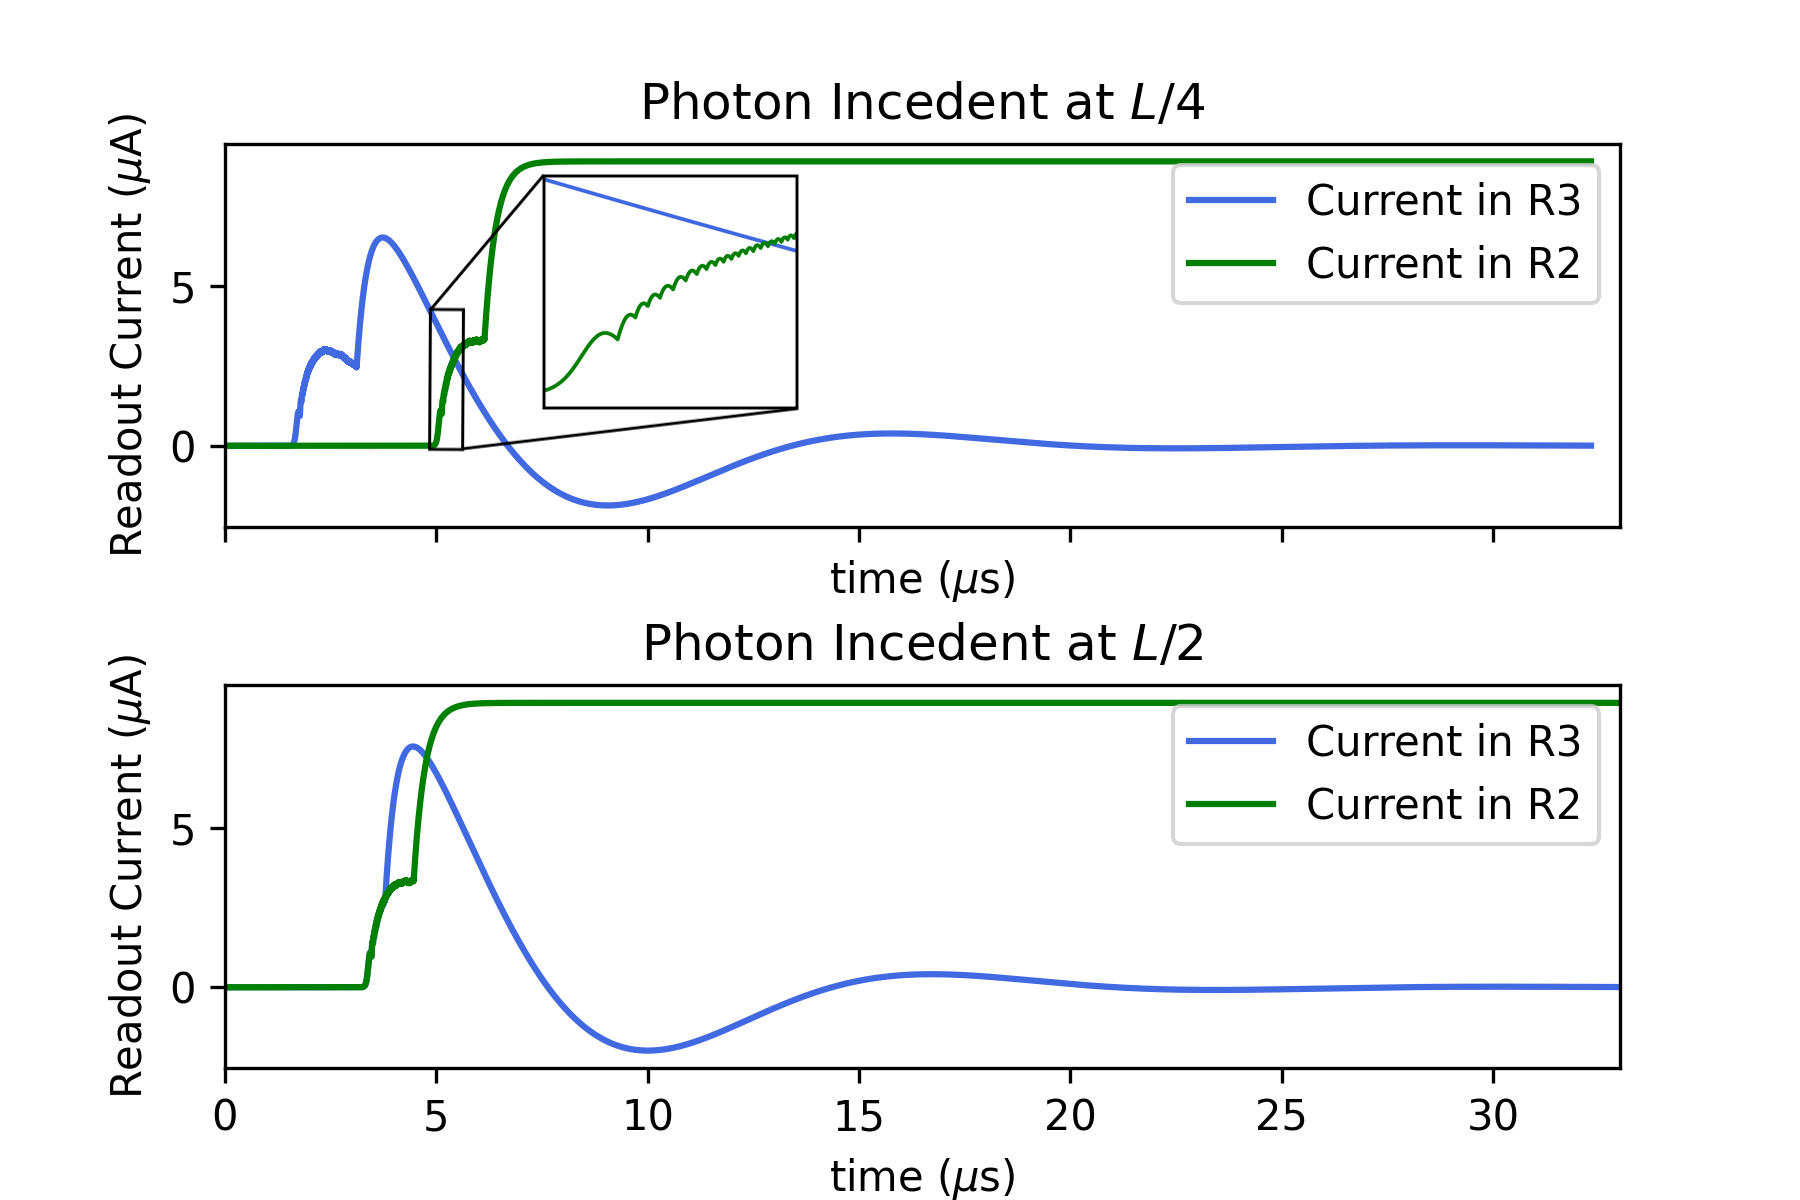
\includegraphics[width=0.5\textwidth]{figs/snspi_out+zoom.png}}
    \caption{Example of a \cf{spice-daemon} generated model for an SNSPI. (a) Setup
    for measuring an SNSPI using differential readout on the RF ports of 2 bias-tees.
    The circular element is the default symbol for \cf{spice-daemon} dynamic model, 
    representing the SNSPI model. (b) Simulation output for a photon incident at
    $x=L/4$ and $x=L/2$ for an SNSPI of length $L$ and 200 discrete elements. 
    In both plots, we see that the SNSPI latches, and the SNSPI carries
    a voltage across it.
    When the pulses form at $L/2$, they take the same amount of time to reach 
    either end of the wire.
    When the photon is incident at $L/4$, the generated pulse closer $x=0$ reaches
    the RF readout port first.}
    \label{fig:snspi_run}
\end{figure}
\todofig[]{SNSPI Working}

Due to hyperparametrization, we have information about the circuit that we can use to
simplify the simulation. For instance, we can replace the entire nanowire model with
one inductor for each ``chunk'' that won't switch. Since \cf{spice-daemon} knows the 
photon locations, we could simplify the netlist. For an SNSPI with $\cf{num\_units}=1000$,
we could make one in every $50$ nanowire elements an actual nanowire, while the
rest are only the inductor portion of the model. This means that only about $5\%$ of the inductors
have the additional hotspot integrator and hotspot resistor. A result of section 
\ref{stability} is our model is more stable and converges faster (we have $3800$ less
highly non-linear behavioral sources and switches from figure \ref{fig:old_nw} and 
the dependency graph collapses
to only one node in figure \ref{fig:dependency_graph}).

\subsection{Arbitrary modeling using scattering parameters}

Modeling experimental equipment, such as a coax cable or bias-tee, involves making a 
lumped approximation of the device and using them in your circuit. 
This type of modeling is sufficient for capturing the qualitative behavior of a device,
but often is not identical to the response of the equipment in the lab.
One solution to this is simulation using the direct scattering parameters - which is
done in programs like Cadence PSpice, but not LTspice \cite{hspice}.

\begin{figure}[h]
    \centering
    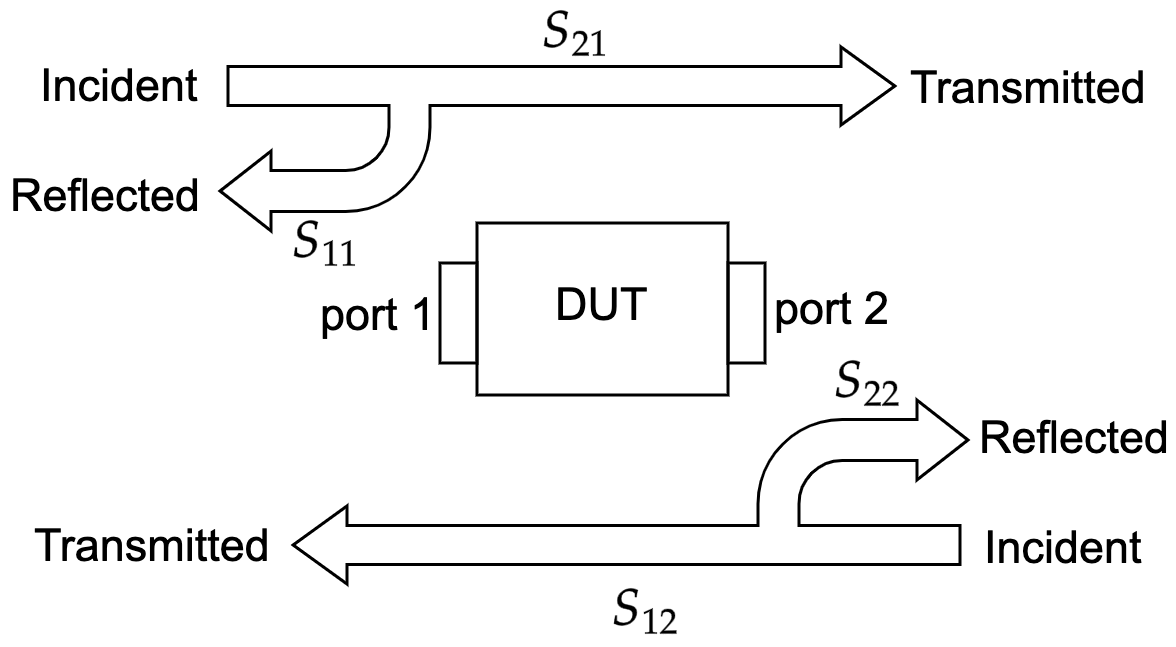
\includegraphics[width=3in]{figs/sxy_diagram.png}
    \caption{Illustration of scattering parameters showcasing the transmitted ($S_{21}$ and $S_{12}$) and reflected ($S_{11}$ and $S_{22}$) signals of a DUT.}
    \label{fig:sxy}
\end{figure}

The scattering parameters (S-parameters) $S_{xy}$ of a $2$-port device describes the
change in magnitude and phase a signal seen at $x$ relative to the signal 
input into port $y$. This notion can be generalize to multiple ports
by taking successive measurements and termination the third port using a
matched load. The S-parameters are frequency dependent and can be described
as an $n\times n$ matrix for a $n$-port device. For passive devices, There exists a 
$1$-to-$1$ mapping from $S$-parameters to $Z$- and $Y$-parameters (impedance 
parameters and admittance parameters respectively).

If we restrict the type of devices we are working with to passive devices,
then we can perform this mapping using voltage-dependent sources in 
LTspice. These sources will use the built-in frequency dependence of b-sources to
define the frequency behavior of the device \cite{microsim}. An accompanying \cf{spice-daemon}
module (\cf{spice-arbnport}) can generate a model with this topology
automatically given the scattering parameters measured for a device.

\subsubsection{2-port model}

\begin{figure}
    \centering
    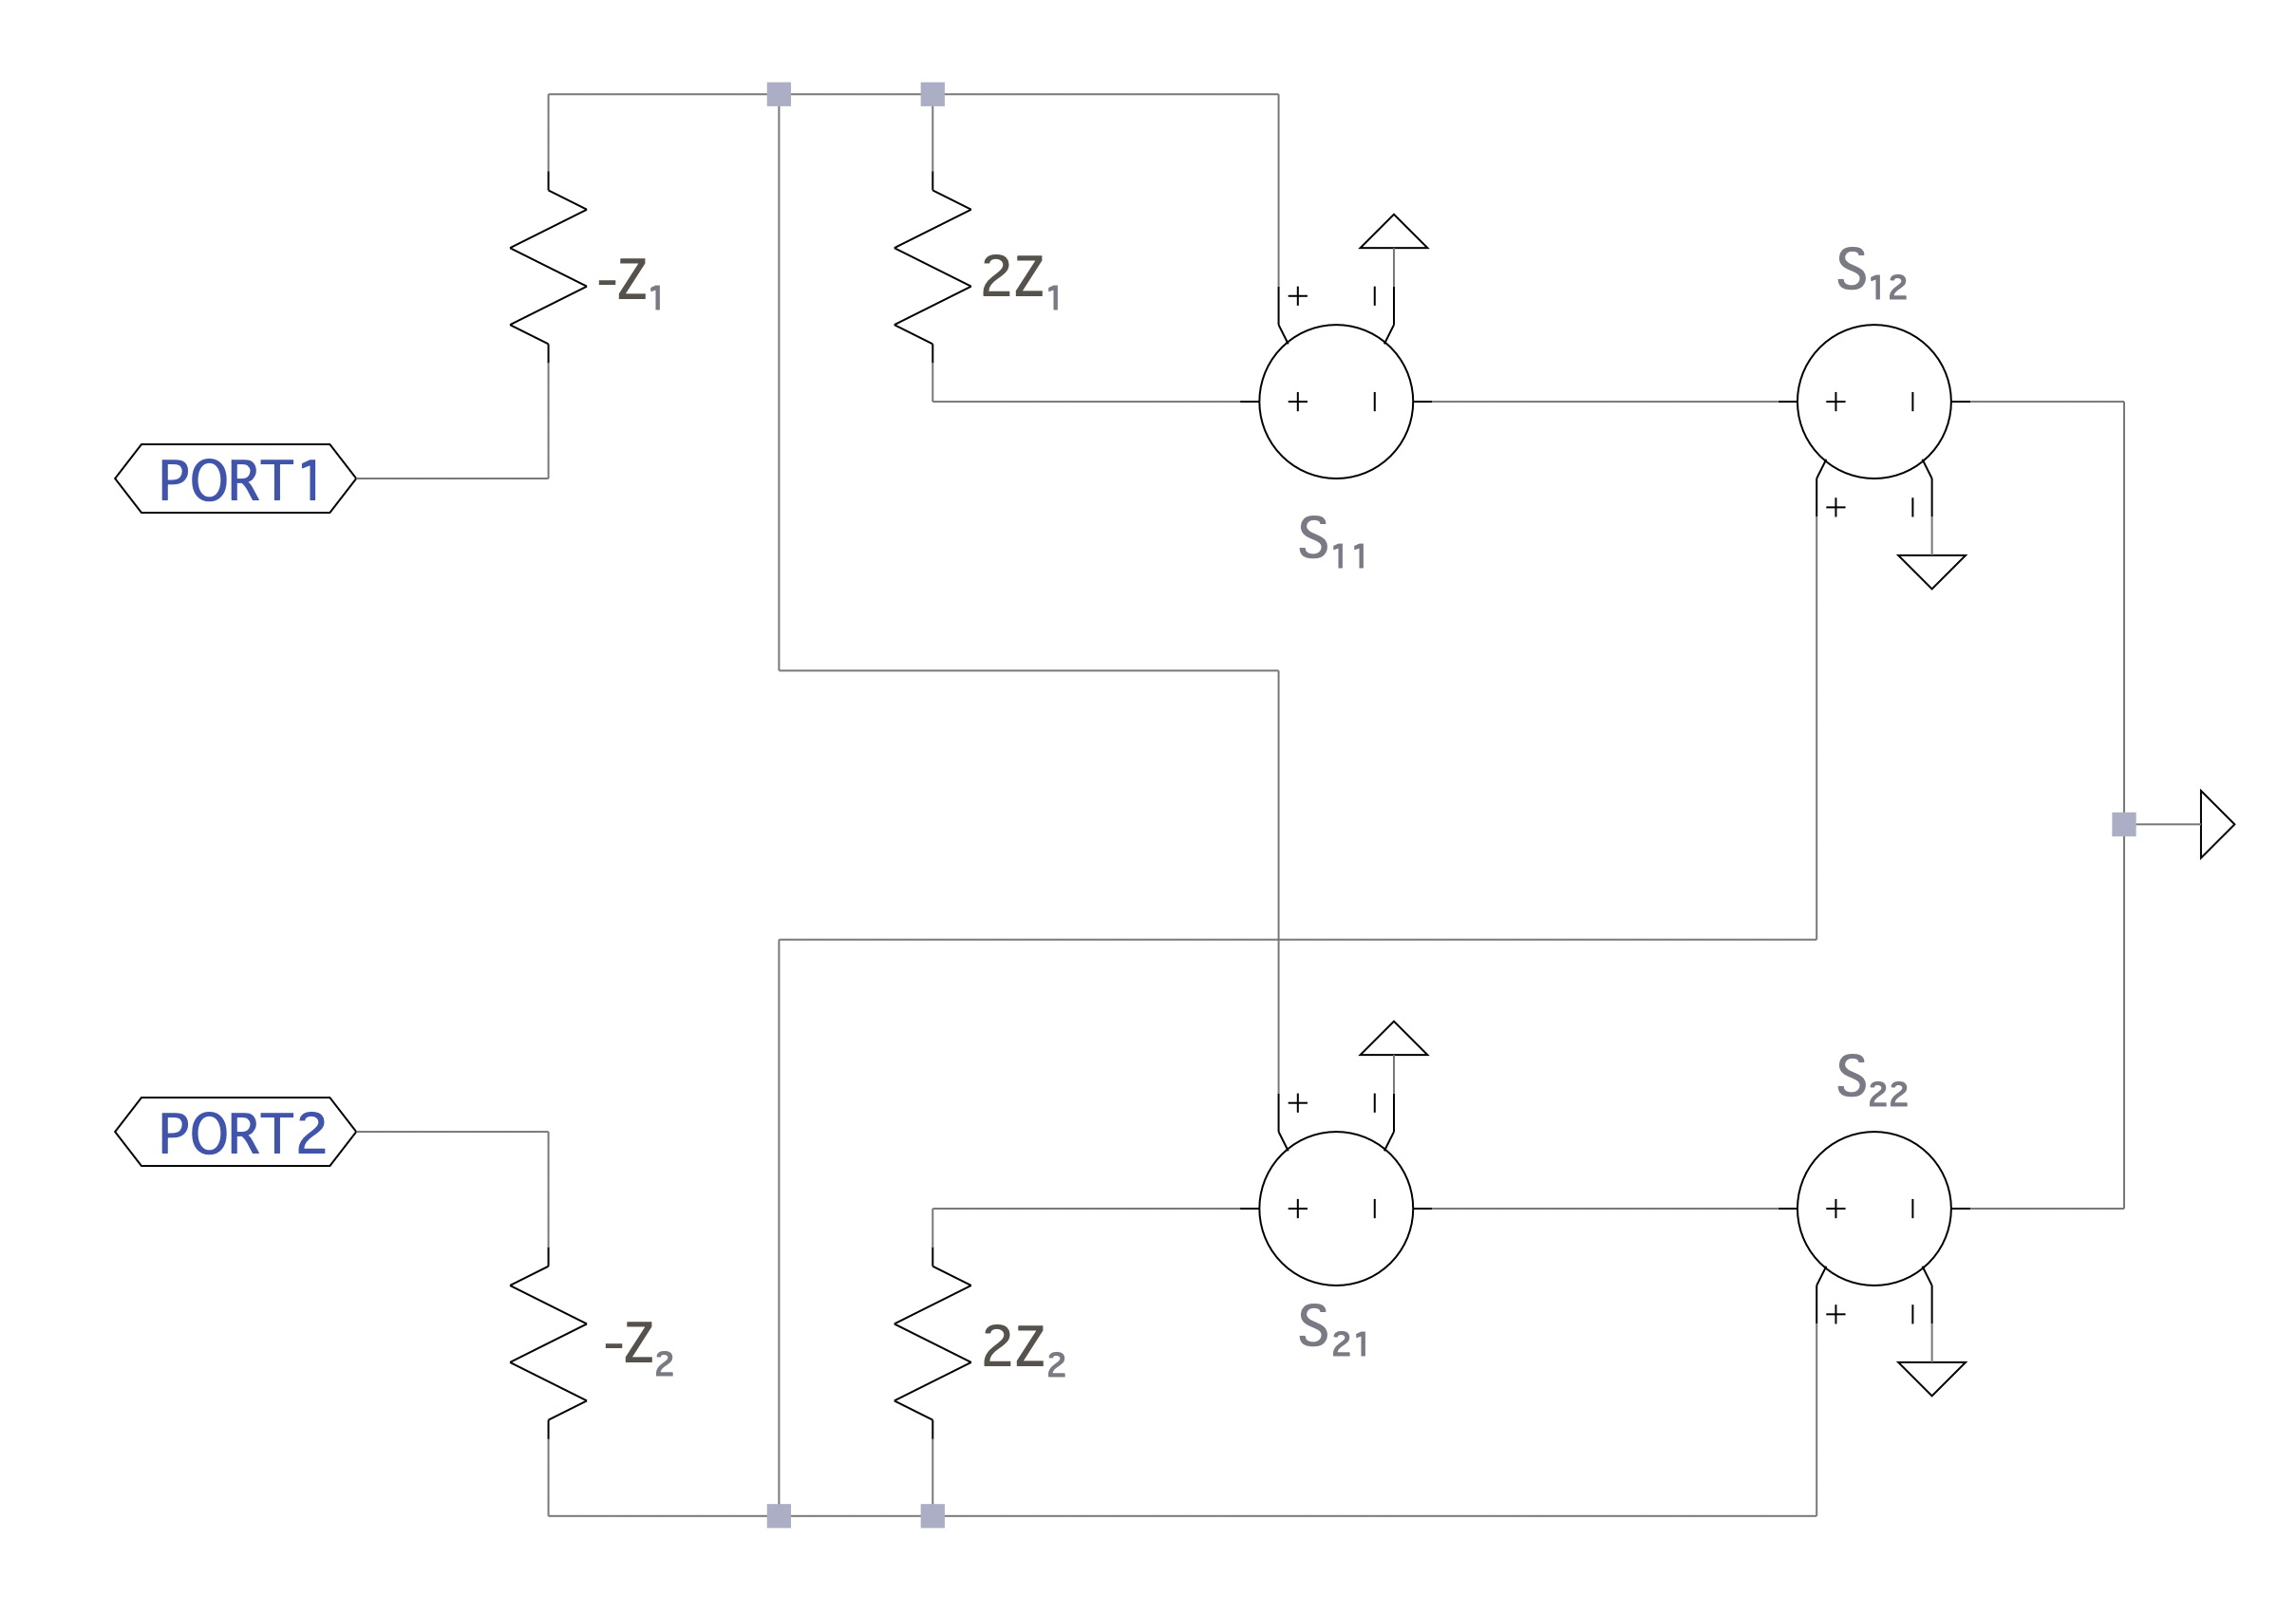
\includegraphics[width=0.8\textwidth]{figs/2port.png}
    \caption{Subcircuit for a 2-port model generated by S-parameters.}
    \label{fig:2port}
\end{figure}

We can model devices with arbitrary frequency-dependent scattering parameters 
using the topology presented in figure \ref{fig:2port} \cite{microsim}. Port 1 and 2 see
an impedance of $Z_1$ and $Z_2$ respectively. Taking $Z_1=Z_2=50\Omega$ and
working with one frequency, each dependent voltage source applies 1 dimension
of the S parameters onto the signal. While figure \ref{fig:2port} uses E-sources,
the actual source uses B-sources (a note on why later in this section).
For instance, if the device is completely
transmissive ($|S_{12}|=|S_{21}|=1$ and $S_{11}=S_{22}=0$) then the sources $S_{21}$
and $S_{12}$ are shorts and an input $V$ at port 1 corresponds to an output of 
magnitude $|S_{11}|\cdot \left|\dfrac{V}{2Z_1-Z_1}\cdot (-Z_1)\right|=|V|$, i.e.
all the power was reflected back. The outputs due to reflection and transmission 
for a given port are independent and as a result (the voltage for each $S_{xy}$ parameter is
added up at port $y$ and the input is at port $x$), you have 8 degrees of freedom in this
network (2 per E-source).

Like other dynamic models, \cf{spice-daemon} generates the netlist for S-parameter-based
devices and adds the S-parameter CSV source to \cf{Simulation.watch\_list}. By specifying
the model name and directory for the CSV in the YAML file, \cf{spice-daemon} will handle model 
generation. Each S-parameter results in generating one b-source that defines a PWL using
a list of 3-tuples. The tuples are encoded as \cf{(frequency, magnitude [in dB], 
phase [in degrees])} by default (this 
can be changed at the expense of slower compilation).

One limitation corresponds to the number of data points, as it increases, the SPICE
gets hung up on generating logic lines. LTspice doesn't document the existence or process
of creating logic lines, however, reverse engineering the binary indicates that logic lines
are related to the process of generating an internal SPICE netlist. This netlist is generated
before any topology checks (and subsequent DC, tran, AC analysis). The logic line assembler runs
on every line separately, and as a result, overloading all the frequency PWL information on
one line speeds up the logic line generation. For $N$ 3-tuples, this takes the processing time
down from $O(N)\xrightarrow[]{} O(1)$ for each source. In practice, for $1.2$ million 3-tuples,
the logic line creation time goes down from above $30$ seconds to below $0.1$ seconds.

The complexity of simulation in the time and frequency domain for LTspice is minimal -- the \cf{freq}
interpolation backend is similar to that used by the \cf{table} directive and \cf{PWL} source mode.
If the logic line creation time is avoided, compilation time is also small, making this method
much more practical for simulating large networks. Using S-parameters, you can simulate an arbitrary
number of ports using a constant-sized network - at the expense of interpolation time and errors. 

\begin{figure}
    \centering

    \subfigure[]{
    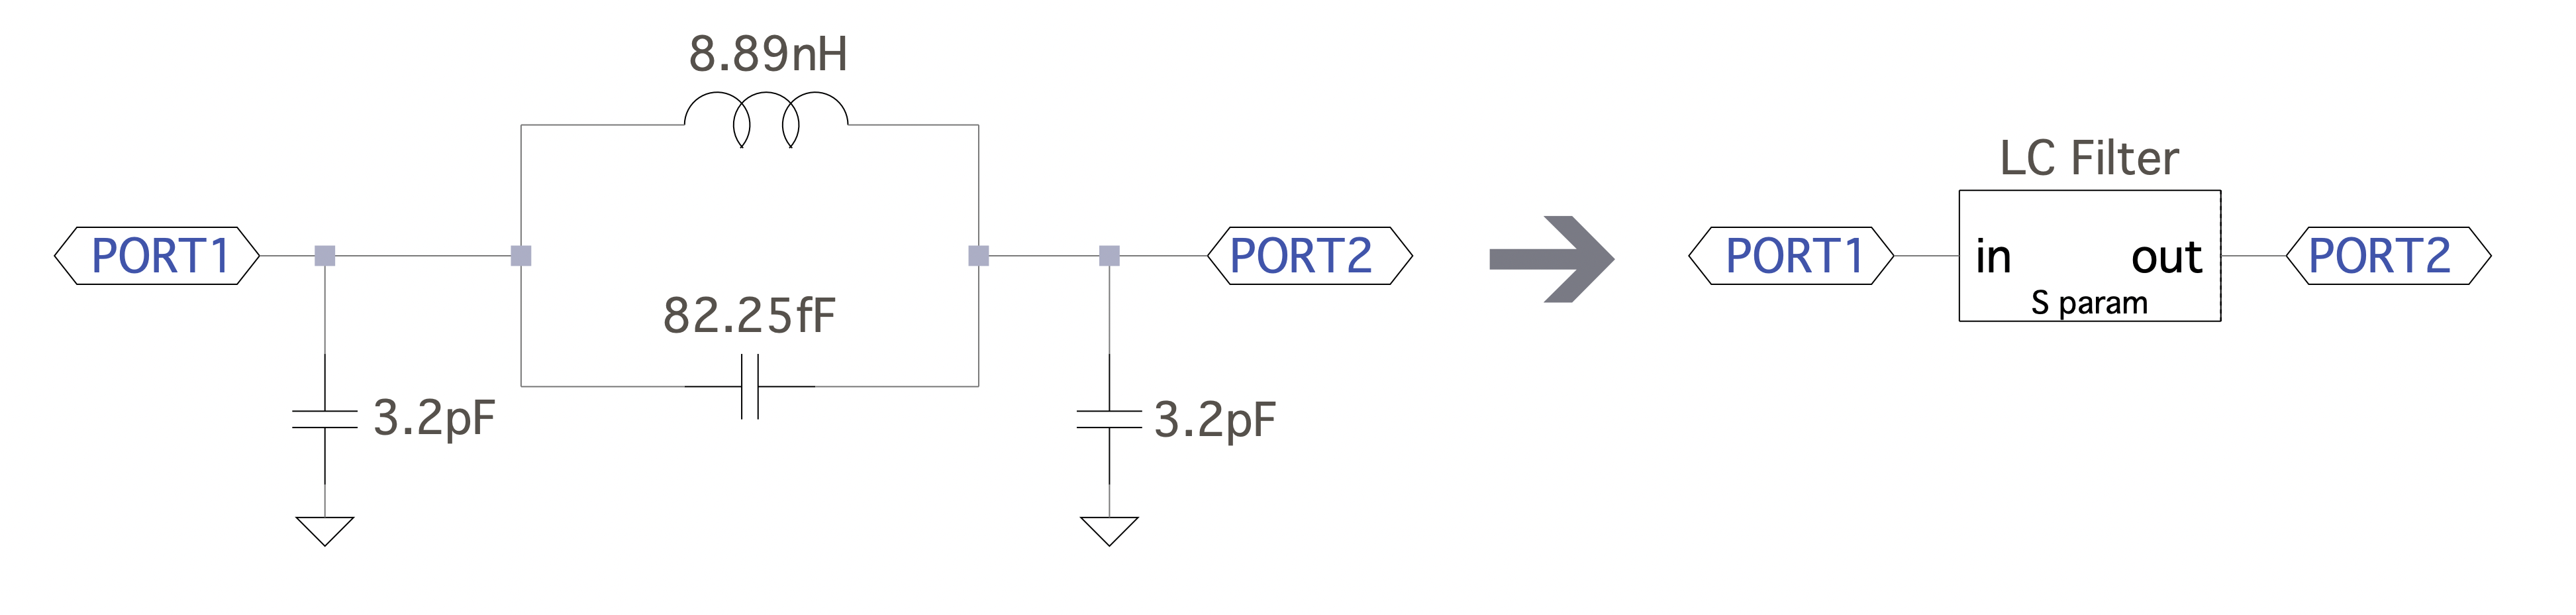
\includegraphics[width=0.8\textwidth]{figs/LC_circ.png}
    \label{fig:LC_circ}
    }
    
    \subfigure[]{
    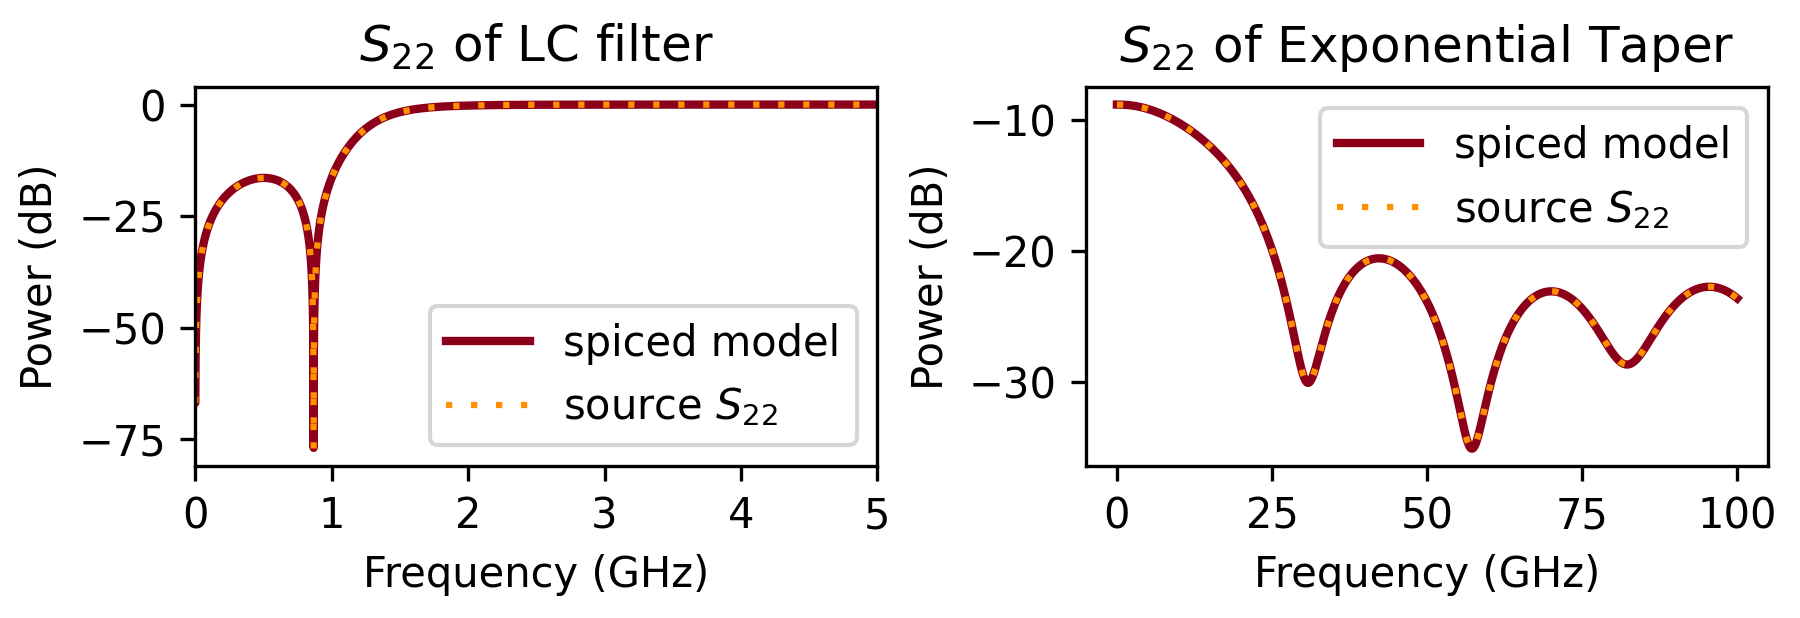
\includegraphics[width=0.8\textwidth]{figs/sparam_run.png}
    \label{fig:sparam_run}
    }
    \caption{(a) Example of an LC subcircuit with 4 elements being encoded into a 1-element
    S-parameter based 2-port device using \cf{spice-daemon}'s dynamic models.
    (b)$S_{22}$ of Analytical vs Scattering Parameter Based Model
    for an LC filter (left) and an exponential taper (right). The solid lines are the S-parameters
    computed from an AC analysis in LTspice using the \cf{spice-daemon} generated 2-port model. The 
    dotted line is the source parameters used by \cf{spice-daemon} to create the model generated
    using \cf{scikit-rf}.}
\end{figure}

Figure \ref{fig:sparam_run} compares the source S-parameters used to generate the dynamic
model to the resultant S-parameters. 
We plot the reflection magnitude computed by the \cf{scikit-rf} package for an LC
filter (figure \ref{fig:LC_circ}) and an exponential taper ($70.8\Omega \xrightarrow[]{} 33.1\Omega$).
We then make a \cf{spice-daemon} model using these
S-parameters (dotted) and plot the calculated S-parameters from the AC analysis.
We see a strong agreement, indicating that the model
functions correctly in simulating the original device. The model is much faster for a linear 
taper in both AC analysis and transient analysis.

\begin{figure}
    \centering
    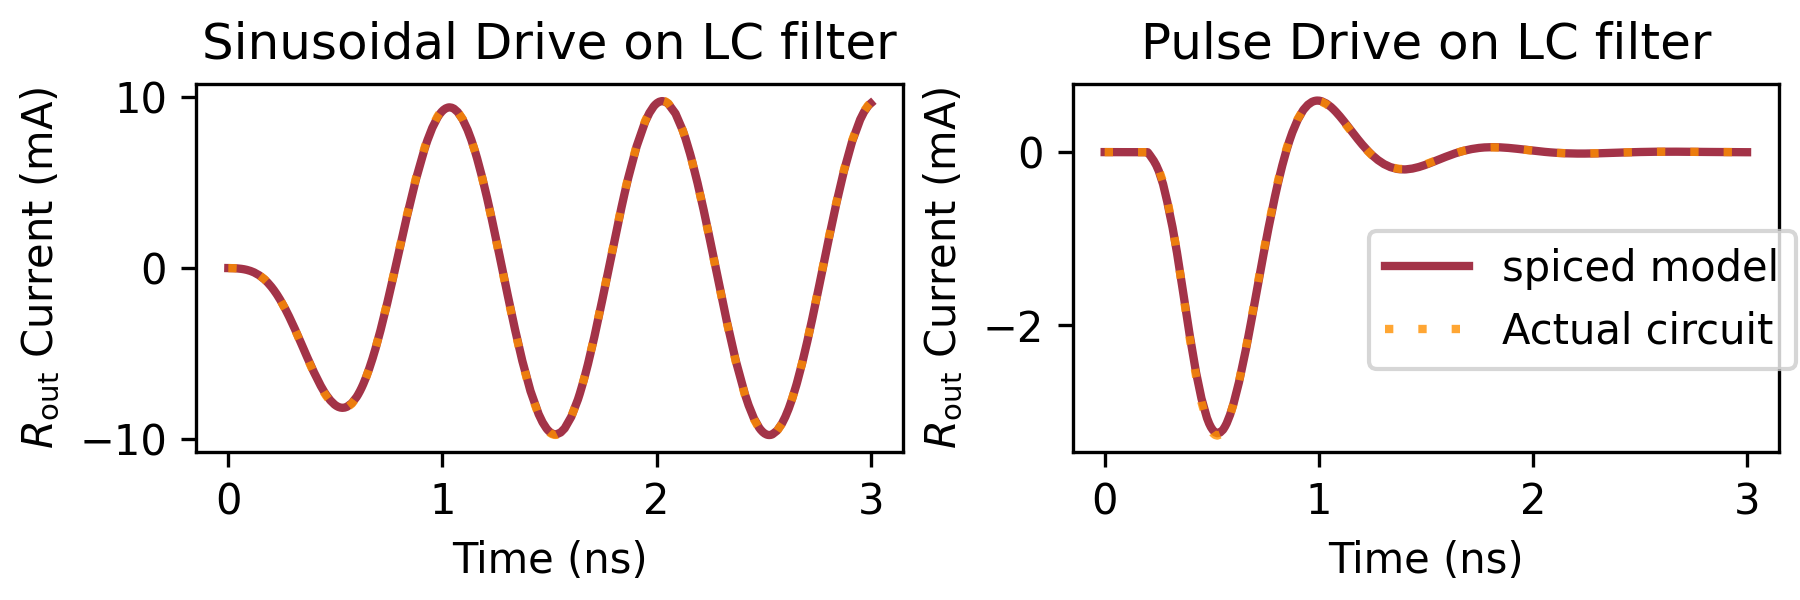
\includegraphics[width=0.8\textwidth]{figs/td_LC.png}
    \caption{Time-domain simulation on the LC filter from figure \ref{fig:LC_circ} comparing the actual circuit to a \cf{spice-daemon} generated dynamic model from only the S-parameters. The S-parameter based model is in agreement with the actual filter's solution for both a sinusoid
    and a pulse input.}
    \label{fig:td_sparam}
\end{figure}

We also show in figure \ref{fig:td_sparam} the agreement in transient analysis by
simulating the \cf{spice-daemon} model vs. the actual LC filter's netlist in LTspice.
We test the response of the LC filter and the \cf{spice-daemon} generated model against
various sine waves frequency ($1$GHz shown) and various width pulses ($0.1$ns shown).
We see a strong agreement in the time domain (the error is bounded below $0.5\%$ for 
the above figure).

The ability to simulate S-parameters directly in a simulation environment is important
for many common topologies used for SNSPD readout. When connecting to a setup, you have to
model every element with a separate model making sure the values in the experiment and simulation
agree. With the ability to use S-parameters directly, you can measure the response of the entire setup
(2 measurements for a 2-port DUT regardless of the number of elements). 
This provides a model that is an accurate reflection of the experiment being 
run (even if the experimental setup has a mistake). This verification
can confirm results that occur even on incorrect setups since we know the exact setup response
and can simulate the device under test with that exact response. 

This can also imply more true-to-experimental setup models, even if the measurement is not repeated.
For instance, characterizing a coax line of a certain length gives an accurate reflection of the coax line
in simulation. Another example is using characterizing filters and running a sweep on them to
decide which filter is the best for a certain application.

\subsubsection{n-port model}

\begin{figure}
    \centering
    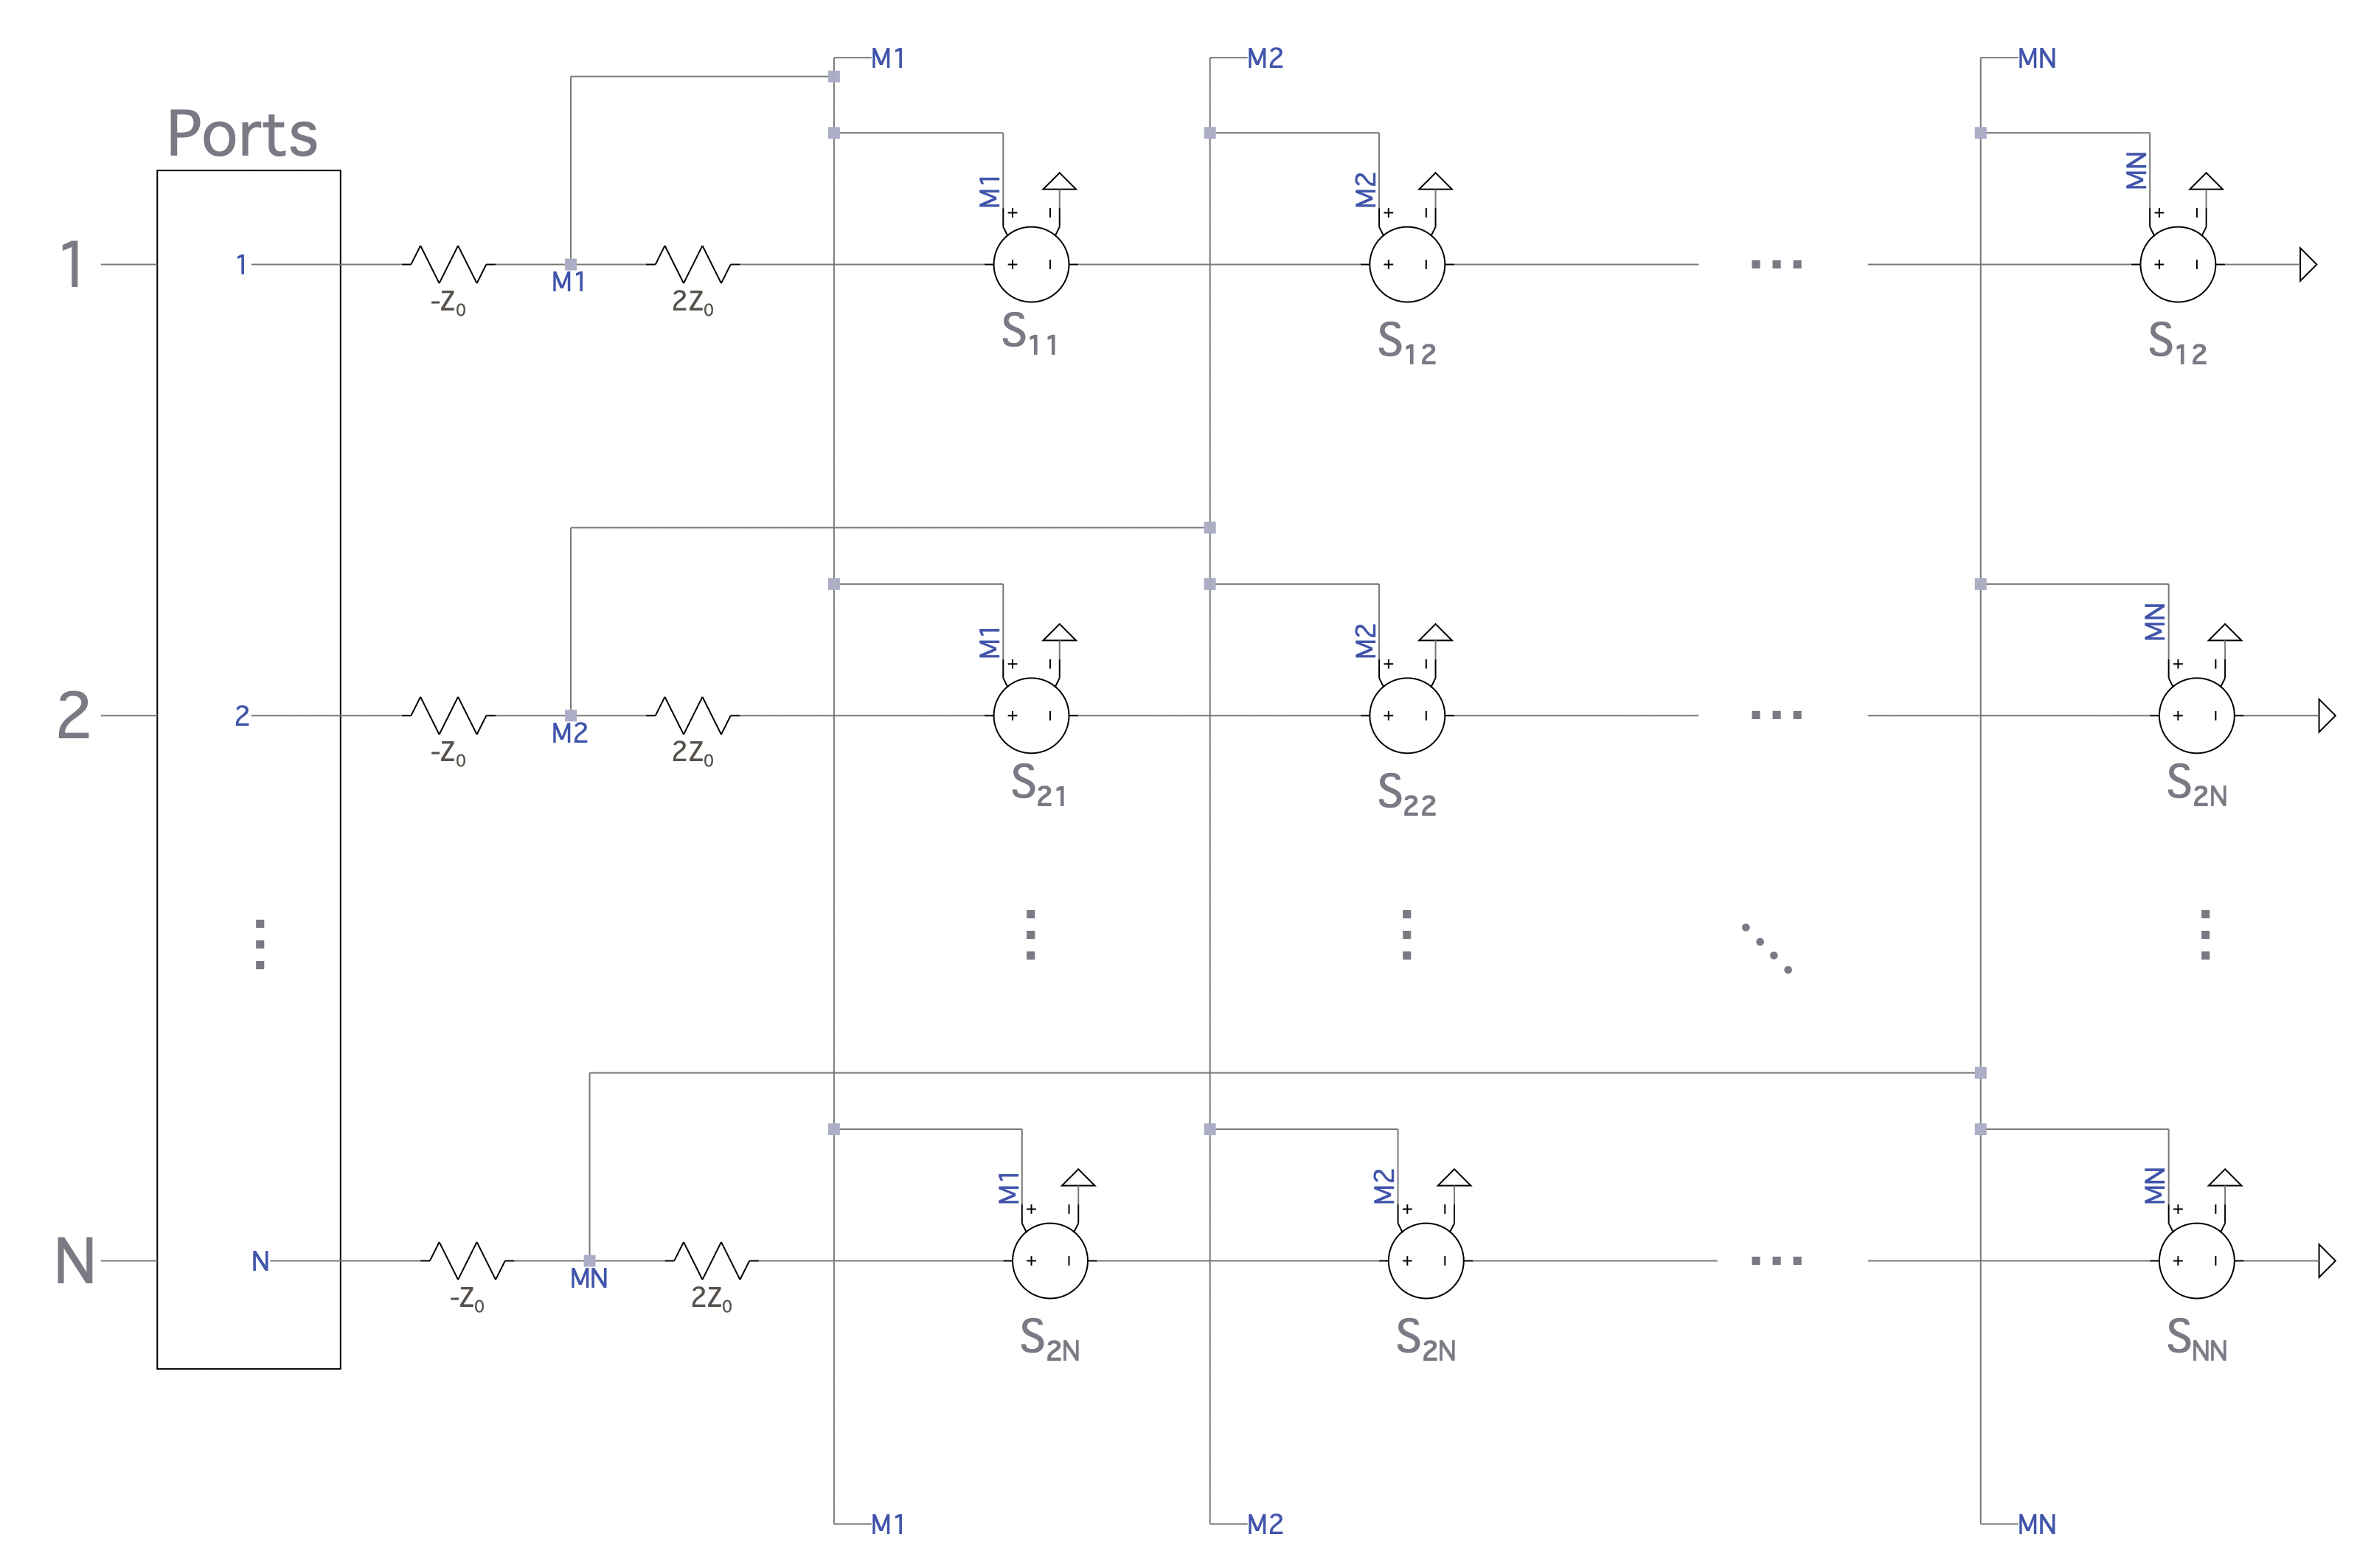
\includegraphics[width=0.8\textwidth]{figs/nport.png}
    \caption{Subcircuit for an $n$-port model to be generated from S-parameters.}
    \label{fig:nport}
\end{figure}

It is also of interest to simulate $n$-port devices, for example, a bias-tee. 
The model can be
scaled to work for $n$-ports as shown in figure \ref{fig:nport}. This scales as $n^2$ with
the number of ports $n$. The actual measurement for parameters $S_{xy}$ can be performed 
by terminating all ports other than $x$ and $y$ with a matched termination. At least
$\frac{n(n-1)}{2}$ sweeps are needed to fully characterize a device \cite{measuring_nport}.

As the number of
ports increases, the number of sources only increases linearly unlike using a circuit 
model. The expression at node \cf{M1} (in figure \ref{fig:nport}) is composed of 
ordering-independent behavioural
sources that can be merged to one source (the order of the individual dependent voltage sources doesn't 
matter and 
therefore the sources can all be merged into one dependent source). The addition of one port results in
adding one more behavioural voltage source at node \cf{M(N+1)}. 
This unfortunately is also coupled with a higher inaccuracy in transient simulations
of varying timesteps. Since these inaccuracies are hard to predict, one option to
extend S-parameter based multi-port devices is to unhook port dependencies that don't
matter. For instance, in a 3-port device where port 0 either reflects the entire
signal or transmits it to port 1, we don't need to include the source on branch \cf{M2}
that is a function of port 0.

\subsubsection{Inaccuracy of S-parameter Modeling in Transient Analysis}

\begin{figure}
    \centering
    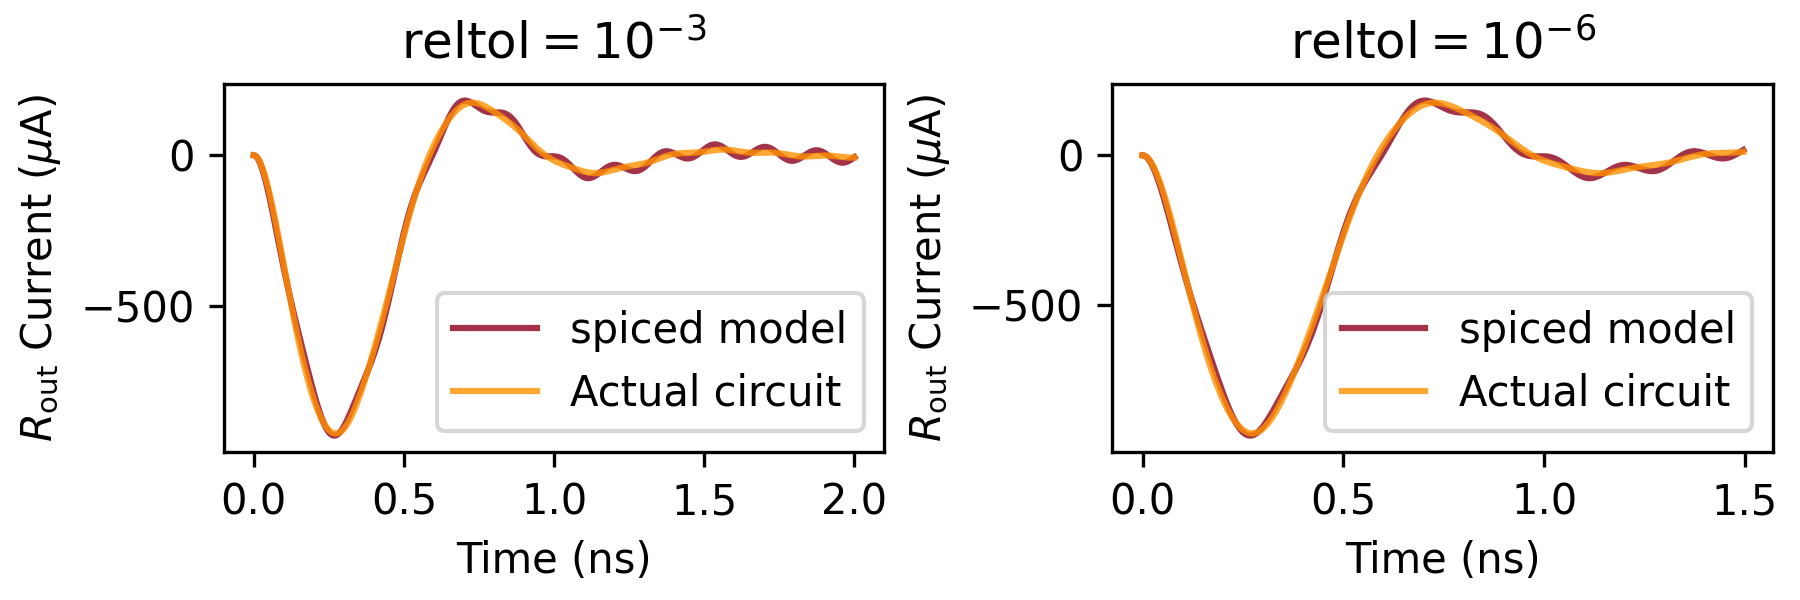
\includegraphics[width=0.8\textwidth]{figs/td_LC_sad.png}
    \caption{Oscillating instability that can be experienced in a transient simulation
    by a S-parameter-based dynamic model generated by LTspice.}
    \label{fig:td_sparam_sad}
\end{figure}

Although the generated models accurately replicate the behavior of the devices in 
AC simulation, they do not consistently perform well in transient analysis.
Simulating S-parameters in a time-domain simulation raises 
time-complexity and accuracy issues due to frequency- and time-domain 
mixing \cite{td-fd-mixing}.
The \cf{spice-daemon} source can be modified to realize a corresponding 
minimal order state-space circuit from a fitted version of the transfer 
function \cite{arb-sparam-spice}.
This method generates linear sub-networks of lumped and non-linear devices
that describes a reduced-order macromodel of an $n$-port device that
are more stable.

Figure \ref{fig:td_sparam_sad} showcases incorrect oscillations that are caused by
using the \cf{spice-daemon} model in transient analysis. Note that the transmittance ($S_{12}$)
for both models is identical, however, this is a result of time/frequency mixing.
These oscillations are present in the actual model but are more attenuated (a factor
of $5$). This effect is seen when the input sinusoid has a frequency of $5.88$GHz,
which corresponds to a sharp pole of the filter's transmittance.

% These oscillations that are strongly coupled to the timestep size and varying other
% parameters, such as number of frequency points doesn't effect the outcome. Figure \ref{fig:td_sparam_sad}
% showcases the oscillations caused by two values for the relative tolerance that
% exhibit different frequency oscillation. Although this oscillation seems similar
% to trapezoidal ringing (discussed in section \ref{stability}), it is a separate
% effect. One quick check can be done using Gear integration which is immune to 
% trapezoidal ringing. The effect is still there with Gear integration 
% (and about doubles in frequency).

\subsection{Post-processing using \cf{spice-daemon} Toolkits}

While LTspice transient simulations are sufficient for characterizing the time behavior of a superconducting 
circuit, an optimized simulation environment should have the ability to post-process the data 
in a meaningful way, producing plots that are familiar to measurements taken in a lab setting.
SPICE transient simulations are optimized to provide
 node voltages as a function of time. However, there may be cases where we are interested in other bases such as the bias current, temperature, frequency bins, or other variables where time is not the independent variable. A widely used measurement for SNSPDs is a PCR (Photon Count Rate) curve, where
the y-axis is the count rate (how many hotspots form on the SNSPD) and the x-axis is the bias current. The ability to replicate that in a simulation environment is an essential step for
design verification and iteration.

Creating a PCR curve requires creating a plot where the x-axis is the bias current used for multiple
periods of simulation time. The y-axis would contain the sum of spikes that the SNSPD has over each period
of time. This sort of rate measurement cannot be performed in LTspice without a complicated secondary circuit
that is bothersome. Using a separate circuit within the simulation is also detrimental to the simulation
performance as it can introduce a non-linear coupling between the counting circuit and the nanowire circuit. 
This coupling can cause the SPICE solver to take longer to run the simulation and cause the nanowire model to
misbehave. The effect of coupling nonlinear circuits is further discussed in Section \ref{stability}.

By hooking a post-processing function to the \cf{WatchDog} class, \cf{spice-daemon} can call this 
function at the end of each simulation. Using \cf{PyLTSpice}'s \cf{LTSpiceRawRead}
function, the contents of LTspice's RAW output file can be dumped into a Python object. This object
separates out each individual trace (voltage at a node, current through a component, time, etc.)
from each simulation step (a single run produced by the \cf{.step} SPICE directive) as separate waveforms. The 
post-processor can then perform any kind of analysis needed from one or multiple simulation runs.
This data is accessible in \cf{spice-daemon} as
\cf{NumPy} arrays and can be extended to new types of post-processing in the same way Dynamic Models can. \cf{spice-daemon} can then update the plot automatically after each simulation run is completed.

The inclusion of post-processing rounds out \cf{spice-daemon} allowing pre- and post-computation
to all happen in an environment optimized for the specific device. While
packages like \cf{PyLTSpice} can be used to manually 
run a script, \cf{spice-daemon}
provides the ability to generate the plots after each simulation invocation automatically.
It also gives a standard way of building post-processing blocks that are directly related
and parametrized by the circuit schematic. 
Post-processing objects can be customized to be device-specific.
For instance, by instantiating a PCR object, \cf{spice-daemon} automatically infers that 
the nanowire circuit is of interest and allows for more compact toolkit specifications.
Since \cf{spice-daemon} has access to the global
variables used in the SPICE simulation, it can also use them in its computation -- a feature
missing from most circuit simulation toolkits.

Toolkits require uniform spacing between datapoints, but SPICE simulators don't have fixed timesteps, 
causing the need for converting data between toolkit invocations. When the RAW file output is parsed
in \cf{spice-daemon}, the \cf{PostProcessing} class (parent to all toolkits) uses extrapolation on these
waveforms. The function \cf{PostProcessing.trace(trace\_name, step)} returns an extrapolated \cf{numpy} 
array of the waveform that has uniform spacing corresponding to the minimum step size. This can
get really large for a smooth signal if all the datapoints are concentrated around one transition
(rising edge of an SNSPD) and can be changed by adding the optional parameter \cf{dt} that defines 
the minimum timestep to extrapolate from.

\subsubsection{IV curves}

IV (current-voltage) curves are an important tool for characterizing the operational margin for a device and ensuring the device was fabricated according to the design. By plotting the current passing through the device as a function of the applied voltage, 
IV curves provide valuable information about the device's behavior: the critical current, 
normal resistance, and the hysteresis margin. Verifying these properties is a common 
indicator that the fabrication process was successful. 
This form of process verification and quality analysis requires an accurate
comparison to provide a useful metric. Being able to simulate the curve for a sample given the desired geometry and comparing
it to the actual fabricated sample provides useful insight into what could have gone wrong during fabrication. 

Given the standardization of IV curves, a good simulation environment for superconducting nanowire based devices
should be able to generate IV plots readily. While a pseudo-DC simulation for the IV curve can be performed
using a slow ramp of bias current, it is bandwidth limited, not an accurate representation of the device physics, 
and takes much longer to perform than doing parallel measurements for the IV curve of a device. Since \cf{spice-daemon}
has the ability to control models and post-analyze signals, we are able to perform an IV curve measurement through
the \cf{spice-daemon} toolkits (post-processing) framework. By running multiple simulations of a PULSE voltage bias source across the nanowire
we can accurately get the DC operating point solution for the nanowire and reconstruct the measured current and voltage
across the nanowire from each simulation into an IV curve. A PULSE source is used instead of a DC 
source for two main reasons: (1) 
simulating hysteresis and (2) the nanowire model is not DC-compatible (discussed in section \ref{stability}).

\todo[inline]{example of IV curve obtained from sd}

\subsubsection{Power Spectral Density}

The Power Spectral Density (PSD) of a signal is a useful tool for designing and studying
superconducting single-photon detectors. It is a 
measure of the power present in a signal as a function of frequency and can provide valuable information about 
the frequency content of the signal. This can be particularly important in nanowires, 
as the PSD can reveal the level of noise present in the system and help identify any 
potential sources of noise that may impact the effective critical current. 
The \cf{spice-daemon} toolkit can be used to generate PSD plots in real-time and can 
optionally incorporate it into the LTspice user interface.

LTspice cannot generate a PSD plot natively and it is unlikely that LTspice
 can generate such a plot without a post-processing framework.
Note that LTspice allows users to plot the Fast Fourier transform (FFT) of a signal but not the 
PSD. \cf{spice-daemon} handles that by taking the FFT in Python and plotting it either in Python's 
plotting package \cf{matplotlib} or by injecting a new node into the RAW output. In addition,
it allows for the use of windowing functions.

\todo[inline]{example of a PSD to replicate noise input}

\subsubsection{Output Methods}

Post-processing modules need to somehow display the signal back to the user. \cf{spice-daemon} handles this
in one of two ways. The preferred method of displaying a plot uses matplotlib to spawn a separate window
that contains all the post-processing plots. The other optional way of doing it is by relying on 
\cf{PyLTSpice}'s \cf{LTSpiceRawWrite} to write new waveforms as specified by the post-processing module.
This method is less preferred as it allows for less customization for plots, it only supports a square
plotting window, shares the x-axis, and doesn't allow for additional markers. As such, unless explicitly
specified, the matplotlib backend is used by default. The matplotlib plotting backend also has multiple 
choices of backends and allows for integration with jupyter notebooks. 

\cf{spice-daemon} provides two options for visualizing post-processing toolkits. The default
option uses \cf{matplotlib} to generate a separate window with all the post-processing
plots. The other option uses \cf{PyLTSpice}'s \cf{LTSpiceRawWrite} to write the waveforms
to the RAW file directly. This option allows for the plots generated to be laid out in the
default LTspice waveform viewer. This method is less flexible, supporting only square 
windows, forces sharing the x-axis, and doesn't support using markers. It also forces
extrapolation at export such that the time axis and exported axis are time-synced.
The \cf{matplotlib} backend on the other hand allows for more customization and 
can be integrated with-in jupyter notebooks and various other \cf{matplotlib} backends.

Post-processing toolkits also allow for saving data in a csv and/or Python objects. 
Toolkits can be used for large-parameter sweeps where the post-processing toolkits
can invoke what the next parameter to search is. For instance, you can implement
gradient descent in LTspice using post-processing toolkits since they have the ability
to hook to modules. Given an arbitrary nanowire circuit, you might want to find the
maximum bias that doesn't switch the wire (accounting for noise). You can use 
the post-processing toolkit to invoke a sequence of LTspice simulations to find
the optimal bias value through gradient descent.

% \subsection{spice-tikz?}